% === Cours de Logique
% === Fichier principal
\usepackage{java}
\usepackage{algoesi}

\title{Logique}
\subtitle{1\textsuperscript{ère} ann\'ee}
\institute[HEB-ESI]{Haute École de Bruxelles --- École Supérieure d'Informatique}    
\date[2013 --- 2014]{Année académique 2013 / 2014}
%\author[]{ \small
 
%  C.~Leruste (clr)
 
%}

\begin{document}
\begin{frame}
\titlepage
\end{frame}

% ===== Inclusion des diffrents chapitres =====
%\include{toc}

% ===== Premier quadrimestre
\section{Algorithmes séquentiels}
%\leconwithtoc

\subsection{Fraction}

\begin{frame}{Exemple}
	Rédiger une marche à suivre détaillée qui explique 
	comment additionner deux fractions~:
	
	\bigskip
	
	\cadre{
		\begin{enumerate}
			\item Rechercher le dénominateur commun des deux fractions
			\item Mettre chaque fraction au même dénominateur
			\item Additionner les numérateurs des deux fractions,
			 ce qui donne le numérateur de la somme
			\item Simplifier la fraction obtenue
		\end{enumerate}
	}
		
	Encore très imprécis. 
	
	Un algorithme proche d'un langage
	de programmation ne devrait mentionner 
	que les opérations élémentaires
	de calcul telles que $+$, -, $*$, $/$.
\end{frame}

\begin{frame}{Exemple plus proche d’un
		programme écrit dans un langage compréhensible par l’ordinateur}
	\cadre{
		\begin{enumerate}
		\item Prendre connaissance du premier numérateur et du premier dénominateur ;
		\item Prendre connaissance du second numérateur et du second dénominateur ;
		\item Multiplier les deux dénominateurs pour obtenir le dénominateur commun ;
		\item Multiplier le premier numérateur par le second dénominateur
			et le second numérateur par le premier dénominateur ;
		\item Additionner ces deux produits pour obtenir le numérateur du résultat ;
		\item Communiquer ce résultat ainsi que le dénominateur commun.
		\end{enumerate}
		}
\end{frame}

\begin{frame}{Langage}
	français~: 
	\begin{itemize}
	\item 
		peut toujours être
		utilisé dans la formalisation d’une première 
		approche de la résolution
		d’un problème.
	
	\item
		trop grande richesse de ce langage en
		comparaison à la pauvreté (mais aussi la rigueur) 
		du langage compris par la machine.
	
	\end{itemize}
\end{frame}

\subsection{Le pseudo-code}

\begin{frame}{Le pseudo-code}
	
	\bigskip
	Le \textbf{pseudo-code} ou \textbf{Langage de Description des
	Algorithmes} (LDA en abrégé) est un langage formel et symbolique
	utilisant :

	\begin{itemize}
	\item
		des \textbf{noms symboliques} destinés à représenter les objets sur
		lesquels s’effectuent des actions ;
	\item
		des \textbf{opérateurs symboliques} ou des mots-clés traduisant les
		opérations primitives exécutables par un exécutant donné ;
	\item
		des \textbf{structures de contrôle} types.
	\end{itemize}
\end{frame}

\subsection{Variables et types}

\begin{frame}{Variables et type}
	\begin{itemize}
		\item les opérations que l’ordinateur devra exécuter portent
			sur des éléments qui sont les \textbf{données} du problème~;
		\item lorsqu’on attribue un \textbf{nom} et un \textbf{type} 
			à ces données, on parle	alors de \textbf{variables}~;
		\item dans un algorithme, une variable conserve
			toujours son nom et son type, mais peut changer de \textbf{valeur}~;
		\item le \textbf{nom} d’une variable permet de la caractériser et de la
			reconnaitre~;
		\item le \textbf{type} d’une variable décrit la nature de son contenu.
	\end{itemize}
\end{frame}

\subsection{Les types autorisés}

\begin{frame}{Types autorisés}
	Dans un premier temps, les seuls \textbf{types} utilisés sont les
	suivants~:
	
	\bigskip
	
	\begin{tabular}{p{1.6cm}|p{11.5cm}}
	\raggedleft  \textbf{entier} &
	 pour les nombres entiers\\
	\raggedleft  \textbf{réel} &
	 pour les nombres réels\\
	\raggedleft  \textbf{caractère} &
	 pour les différentes lettres et caractères \\
	{~} & (par exemple ceux qui apparaissent sur un \\
	{~} & clavier~: ‘a’, ‘1’, ‘\#’, etc…)\\
	\raggedleft  \textbf{chaine} &
	pour les variables contenant plusieurs
	caractères\\
	{~} & ou aucun (la chaine vide) \\
	{~} &	(par exemple : "Bonjour", "Bonjour le monde",  \\
	{~} &	"a", "", etc.)
	\\
	\raggedleft  \textbf{booléen} &
	 les variables de ce type ne peuvent valoir que
	\textbf{vrai} ou \textbf{faux}\\
	\end{tabular}
\end{frame}

\begin{frame}{Exercice}
	Quel(s) type(s) de données utiliseriez-vous 
	pour représenter 
	\begin{itemize}
		\item une date du calendrier ?
		\item un moment dans la journée ?
		\item le prix d'un produit en grande surface ?
		\item votre nom ?
		\item vos initiales ?
		\item votre adresse ?
	\end{itemize}	
\end{frame}

\subsection{Déclaration de variables}

\begin{frame}{Déclaration de variables}
	La déclaration d’une variable est l’instruction 
	qui définit son nom et son type.
	\cadre{
		\begin{pseudo}
			\Declare{num1, num2}{entiers}
		\end{pseudo}
	}
	
	\bigskip
	
	L’ensemble des instructions de la forme

	\cadre{
	\begin{pseudo}
	\Declare{variable1, variable2,\ldots}{type}
	\end{pseudo}
	}

	forme la partie d’un algorithme nommée 
	\textbf{déclaration des variables}. 
\end{frame}

\begin{frame}{Déclaration de variables}
	La déclaration des informations apparaitra toujours 
	\begin{itemize}
	\item 
	en \textbf{début} d’algorithme, 
	\item
	ou dans un bloc annexe appelé 
	\textbf{dictionnaire des variables} 
	\item
	ou encore \textbf{dictionnaire des données}.
	\end{itemize}
\end{frame}

\begin{frame}{Déclaration de variables~: exemple}
	Pour l’algorithme des fractions, la déclaration des
	informations pourrait être la suivante :

	\cadre{
	\begin{pseudo}
	\Declare{num1, den1, num2, den2, numRes, denRes}{entiers}
	\end{pseudo}
	}

	avec la signification suivante :

	\begin{itemize}
	\item
		\textit{num1 (num2)}~: le numérateur 
		de la première (seconde) fraction ;
	\item
		\textit{den1 (den2)}~: le dénominateur 
		de la première (seconde) fraction ;
	\item
		\textit{numRes (denRes)}~:
		le numérateur (dénominateur) du résultat.
	\end{itemize}
\end{frame}

\begin{frame}{Déclaration de variables}
	\begin{itemize}
	\item
	Lors de la déclaration d’une variable, celle-ci n’a pas de
	valeur ! 
	\item
	Ce sera l’instruction d’\textbf{affectation} 
	qui va servir à donner un contenu aux variables
	déclarées. 
	\item
	En logique, nous n’envisageons pas d’\textit{affectation par
	défaut}
	\end{itemize}
\end{frame}

\subsection{Comment nommer correctement une variable ?}

\begin{frame}{Comment nommer correctement une variable ?}
	Un nom de variable
	\begin{itemize}
		\item est suffisamment court tout en restant explicite
		\item ne prête pas à confusion
		\item tient compte des limitations imposées par les
			langages de programmation
	\end{itemize}
\end{frame}

\begin{frame}{Comment nommer correctement une variable ?}
	Quelques règles et limitations traditionnelles dans les langages
	de programmation:

	\bigskip
	
	\begin{itemize}
	\item 
		Un nom de variable est généralement une suite de caractères
		alphanumériques d’un seul tenant (pas de caractères blancs) et ne
		commençant jamais par un chiffre. Ainsi \textit{x1} est
		correct mais non \textit{1x}. 
	\end{itemize}
\end{frame}

\begin{frame}{Comment nommer correctement une variable ?}
	\begin{itemize}
	\item 
		Pour donner un nom composé à une variable, on peut utiliser le 
		\textit{underscore} (par ex. premier\_numérateur) mais on
		déconseille d’utiliser le signe «~–~» qui est plutôt réservé à la
		soustraction. 
	
	\bigskip
	
	\item 
		Une alternative à l’utilisation du tiret bas pour l’écriture de noms de
		variables composés est la notation «~chameau~» (\textit{camelCase} en
		anglais), qui consiste à mettre une majuscule au début des mots
		(à partir du deuxième), par exemple
		\textit{premierNombre} ou
		\textit{dateNaissance}.
		\end{itemize}
	\end{frame}

\begin{frame}{Comment nommer correctement une variable ?}
	\begin{itemize}

	\item
		Les indices et exposants sont proscrits (par ex.
		\textit{$x_1$},
		\textit{$z_6$} ou
		\textit{$m^2$)}
		
	\bigskip
	
	\item
		On n'utilisera pas non plus les 
		mots-clés du langage/pseudo-code (tels que
		\textbf{\textsf{lire}}, 
		\textbf{\textsf{afficher}}, 
		\textbf{\textsf{pour}}…)
		
	\bigskip
	
	\item
		Certains langages n’autorisent pas les caractères accentués (tels que
		\textit{à, ç, ê, ø,} etc.) ou les lettres des alphabets non latins
		(tel que ${\Delta}$) mais d’autres oui ; certains font la distinction
		entre les minuscules et majuscules, d’autres non. En logique, nous
		admettons dans noms de variables les caractères accentués du français,
		par ex~: durée, intérêts, etc.
	\end{itemize}
\end{frame}

\begin{frame}{Exercices}
	Déclarer le(s) variable(s) permettant de représenter 
	\begin{itemize}
		\item la date d'anniversaire de quelqu'un.
		\item l'heure de début, l'heure de fin et	l'objet d'un rendez-vous.
	\end{itemize}
\end{frame}

\subsection{Opérateurs et expressions}

\begin{frame}{Opérateurs et expressions}
	Les opérateurs agissent sur les variables et les constantes pour former
	des \textbf{expressions}. 
	
	\bigskip
	
	Une expression est donc une combinaison
	\textbf{cohérente} de variables, de constantes et d’opérateurs,
	éventuellement accompagnés de parenthèses.
\end{frame}

\begin{frame}{Opérateurs arithmétiques élémentaires}
	Ce sont les opérateurs binaires bien connus :
	
	\bigskip
	
	\begin{tabular}{p{1.6cm}|p{11.5cm}}
	\raggedleft  \textit{+} & addition\\
	\raggedleft  \textit{-} & soustraction\\
	\raggedleft  \textit{*} & multiplication\\
	\raggedleft  \textit{/} & division réelle\\
	\raggedleft  \textit{DIV} & division entière\\
	\raggedleft  \textit{MOD} & reste de la division entière\\		
	\end{tabular}
	
	\bigskip
	
	Ils agissent sur des variables ou expressions à valeurs entières ou
	réelles. 
	
\end{frame}

\begin{frame}{Opérateurs arithmétiques élémentaires}
	\begin{itemize}
		\item
		Plusieurs opérateurs peuvent être utilisés pour former des
		expressions plus ou moins complexes, en tenant compte des règles de
		calcul habituelles, notamment la priorité de la multiplication et de la
		division sur l’addition et la soustraction. 
		
	\bigskip
	
		\item
		Il est aussi permis	d’utiliser des parenthèses.
	\end{itemize}
\end{frame}

\begin{frame}{Fonctions mathématiques complexes}
	\begin{itemize}
	\item
	L’élévation à la puissance sera notée \textit{**} ou
	\textit{\^{}} . 
	
	\bigskip
	
	\item
	La racine carrée d’une variable x s'écrira
	$\sqrt{x}$ \textit{.} 
	
	Attention, pour ce dernier, de veiller
	à ne l’utiliser qu’avec un radicant positif !

	\bigskip
	
	\item
	On se permettra d'utiliser les autres
	fonctions mathématiques sous leur forme la plus courante
	(exemples~:	$sin(x)$, $tan(x)$, $log(x)$, $exp(x)$, ...)
	\end{itemize}
\end{frame}

\begin{frame}{Fonctions mathématiques complexes}
	\textbf{Exemple} : 
	$(-b+\sqrt{(b\ast \ast 2-4\ast a\ast c)})/(2\ast a)$
	
	\bigskip
	
	Mais on peut aussi accepter la notation mathématique usuelle
	\begin{center}
	$\frac{-b+\sqrt{b^{2}-4\ast a\ast c}}{2\ast a}$ 
	\end{center}
	
	\bigskip

	Pourquoi ne pas avoir écrit «~\textit{4ac}~» et
	«~\textit{2a}~» ?
\end{frame}

\begin{frame}{Opérateurs de comparaison}

	Ils agissent sur des variables numériques ou des
	chaines et donnent un résultat booléen.

	\bigskip

	\begin{tabular}{p{1.6cm}|p{11.5cm}}
	\raggedleft  \textit{=} & égal\\
	\raggedleft  \textit{{\textless}{\textgreater}}
		ou \textit{${\neq}$} &  différent de\\
	\raggedleft  \textit{\textless} & (strictement) plus petit que\\
	\raggedleft  \textit{\textgreater} & (strictement) plus grand que\\
	\raggedleft  \textit{${\leq}$} & plus petit ou égal\\
	\raggedleft  \textit{${\geq}$} & plus grand ou égal\\
	\end{tabular}
	
	\bigskip

	Pour les chaines, c'est l’ordre alphabétique qui
	détermine le résultat (par exemple
	\textit{{\textquotedbl}milou{\textquotedbl} {\textless}
	{\textquotedbl}tintin{\textquotedbl}} est \textbf{vrai} de même que
	\textit{{\textquotedbl}assembleur{\textquotedbl}
	}\textit{${\leq}$}\textit{
	{\textquotedbl}java{\textquotedbl}})
	
\end{frame}
	
\begin{frame}{Opérateurs logiques}

	Ils agissent sur des expressions booléennes 
	pour donner un résultat du même type.
	
	\bigskip

	\begin{tabular}{p{1.6cm}|p{11.5cm}}
	\raggedleft  \textit{NON} & négation\\
	\raggedleft  \textit{ET} & conjonction logique\\
	\raggedleft  \textit{OU} & disjonction logique\\
	\end{tabular}
\end{frame}

\begin{frame}{Opérateurs logiques}
	\begin{itemize}
	\item
	\textbf{cond1 ET cond2} n’est vrai que lorsque
	les deux conditions sont vraies. 
	
	\item
	\textbf{cond1 OU cond2} est
	toujours vrai, sauf quand les deux conditions sont fausses.

	\item
	Parenthèser dans le cas de combinaisons de ET et de
	OU : 
	
	\textbf{(cond1 ET cond2) OU cond3} étant différent de
	
	\textbf{cond1 ET (cond2 OU cond3).} 
	
	\item
	En cas d'oubli de parenthèses,
	\textbf{\textit{ET} est prioritaire sur le \textit{OU}}.
	\end{itemize}
\end{frame}

\begin{frame}{Opérateurs logiques}

	Pour un booléen \textit{ok}~: 
	
	\begin{itemize}
	\item
	\textbf{ok = faux} est équivalent à \textbf{NON ok},
	\item
	\textbf{ok = vrai} est équivalent à \textbf{ok} et 
	\item
	\textbf{NON NON ok} est équivalent à \textbf{ok}.
	\end{itemize}
	Dans les trois cas, nous préconiserons la seconde écriture.
\end{frame}

\begin{frame}{Évaluation complète et court-circuitée}

	On définit deux modes d’évaluation des opérateurs \textit{ET}
	et \textit{OU} :

	\begin{itemize}
	\item{l’évaluation \textit{complète}}
	\item{l’évaluation \textit{court-circuitée}}
	\end{itemize}
	Dans le cadre de ce cours, nous opterons pour la deuxième 
	interprétation.
	
	\bigskip
	
	Exemple~: considérons	l’expression 
		{$n {\neq} 0 \ ET \  m/n > 10$}.
\end{frame}
		
\begin{frame}{Manipuler les chaines}
	Pour les chaines, nous allons introduire quelques notations
	qui vont nous permettre de les manipuler plus facilement.

	\begin{itemize}
	\item \textit{long(maChaine)}
		donne la taille (le nombre de caractères) de la chaine 
		\textit{maChaine}.
	\item \textit{car(maChaine,pos)}
		donne le caractère en position \textit{pos} 
		(à partir de 1) dans la chaine \textit{maChaine}.
	\item \textit{concat(maChaine1,maChaine2)}
		concatène les chaines \textit{maChaine1} 
		et \textit{maChaine2}.
		(ex: \textit{concat("Bon","jour")} donne \textit{"Bonjour"})
	\end{itemize}
\end{frame}

\begin{frame}{Manipuler les caractères}

		Introduisons également quelques notations pour les caractères.

		\begin{itemize}
		\item \textit{chaine(car)} transforme le caractère \textit{car} en une chaine de taille 1.
		\item \textit{estLettre(car)} est vrai si le caractère \textit{car} est une lettre
			(idem pour \textit{estChiffre}, 
			\textit{estMajuscule}, 
			\textit{estMinuscule}).
		\item \textit{majuscule(car)} donne la majuscule de la lettre \textit{car}
			(idem pour \textit{minuscule}).
		\item \textit{numLettre(car)} donne la position de \textit{car} dans l'alphabet (ex: \textit{numLettre('E')} donne 5, 
		idem pour \textit{numLettre('e')}).
		\item \textit{lettre(num)} l'inverse de la précédente (ex: \textit{lettre(4)} donne le caractère 'D').
	\end{itemize}
\end{frame}

\subsection{L’affectation d’une valeur à une variable}
\begin{frame}{Affectation externe}
	L’\textbf{affectation externe} est la primitive qui permet de recevoir de
	l’utilisateur, au moment où l'algorithme se déroule,
	une ou plusieurs valeur(s) et de les affecter à des variables en
	mémoire.

	\bigskip
	
	\cadre{
	\begin{pseudo}
	\Read liste\_de\_variables\_à\_lire
	\end{pseudo}
	}
\end{frame}

\begin{frame}{Affectation interne }
	On parle d’affectation interne lorsque la valeur d’une variable est
	«~calculée~» par l’exécutant de l’algorithme lui-même à partir de
	données qu’il connait déjà :

	\bigskip
	
	\cadre{
	\begin{pseudo}
	\Let nomVariable \Gets expression
	\end{pseudo}
	}
	
	\bigskip
	
	Par exemple~:

	\cadre{
	\begin{pseudo}
	\Let somme \Gets nombre1 + nombre2
	\Let denRes \Gets den1 * den2
	\Let cpt \Gets cpt + 1
	\Let delta \Gets b**2 – 4*a*c
	\Let test \Gets a < b \RComment pour une variable logique
	\Let maChaine \Gets "Bon"
	\Let uneChaine \Gets concat(maChaine, "jour")
	\end{pseudo}
	}
\end{frame}

\begin{frame}{Affectation}
	Il est de règle que le résultat de l’expression à droite du signe
	d’affectation ($\gets$) soit de
	même type que la variable à sa gauche. On tolère certaines exceptions~:
	\begin{itemize}
	\item
		\textit{varEntière}{ $\gets$ }\textit{varRéelle} : 
		dans ce cas le contenu de la variable sera la valeur \textbf{tronquée}
		de l’expression réelle. 
		
		Par exemple si «~\textit{nb}~» est
		une variable de type entier, son contenu après l’instruction
		«~\textit{nb}{ $\gets$ }\textit{$15/4$}~» 
		sera 3
	\item 
		\textit{varRéelle}{ $\gets$ }\textit{varEntière} :
		ici, il n'y a pas de perte de valeur.
	\item 
		\textit{varChaine}{ $\gets$ }\textit{varCaractère} : 
		
		équivalent à \textit{varChaine}{ $\gets$ }\textit{chaine(varCaractère)}.
		
		Le contraire n'est évidemment pas accepté.
	\end{itemize}
\end{frame}

\begin{frame}{Affectation}
	\begin{itemize}
	\item 
		Seules les variables déclarées peuvent être affectées, que ce soit par
		l’affectation externe ou interne!
	\item 
		Nous ne mélangerons pas la déclaration d’une variable et son
		affectation interne dans une même ligne de code, donc pas
		d’instructions hybrides du genre 
		\textsf{x}{ $\gets$ }\textit{2 : entier} ou encore 
		\textsf{x~: entier(0)}.
	\item 
		Pour l’affectation interne, toutes les variables apparaissant dans
		l'\textit{expression} doivent avoir été affectées
		préalablement. Le contraire provoquerait un arrêt de l’algorithme.
	\end{itemize}
	
\end{frame}

\subsection{Communication des résultats}
\begin{frame}{Communication des résultats}

	\cadre{
	\begin{pseudo}
	\Write \textit{expression} ou \textit{liste de variables séparées par des virgules}
	\end{pseudo}
	}

	\bigskip
	
	signifie que la valeur d’une expression (ou celles des différentes
	variables mentionnées) sera fournie à l’utilisateur (par exemple par un
	affichage à l’écran ou par impression sur listing via l’imprimante,
	etc\dots).
	
	\bigskip
	
	Comme pour l’affectation interne, on ne peut \code{afficher}
	que des expressions dont les variables qui la composent ont été 
	affectées préalablement.
\end{frame}

\subsection{Structure générale d’un algorithme}
\begin{frame}{Structure générale d’un algorithme}
	La traduction d’un algorithme en pseudo-code constituera le contenu d’un
	\code{module}. 
	
	\bigskip
	
	Un \code{module} contient donc la solution
	algorithmique d’un problème donné (ou d’une de ses parties). 
	
	\bigskip
	
	Sa structure générale sera la suivante :
	
	\bigskip
	
	\cadre{
	\begin{pseudo}
	\Module{nomDuModule}{}{}
		\Stmt \textit{déclaration des variables et constantes utilisées dans le module}
		\Stmt \textit{lecture des données}
		\Stmt \textit{instructions utilisant les données lues}
		\Stmt \textit{communication des résultats}
	\EndModule
	\end{pseudo}
	}		
	
	\bigskip
	
	Comme pour les variables, le nomDuModule devra être approprié au contenu.
\end{frame}

\begin{frame}{Fraction(suite)}
	Réécrivons l’algorithme d’addition de fractions décrit
	en début de chapitre~:

	\bigskip
	
	\cadre{
	\begin{pseudo}
	\Module{additionnerFractions}{}{}
		\Declare{num1, den1, num2, den2, numRes, denRes}{entiers}
		\Read num1, den1, num2, den2
		\Let denRes \Gets den1 * den2
		\Let numRes \Gets num1*den2 + num2*den1
		\Write numRes, "/", denRes
	\EndModule
	\end{pseudo}
	}
	
	\bigskip
	
	\textbf{Remarque~:}
	rappelons que la fraction affichée n'est sans doute pas simplifiée. 
	
	Nous n'avons pas encore tous les atouts suffisants pour réaliser 
	cela à ce niveau. Patience !
\end{frame}

\subsection{Commenter un algorithme}
\begin{frame}{Commenter un algorithme}
	On n’insistera jamais assez sur la nécessité de \textbf{documenter} un
	algorithme en y insérant des \textbf{commentaires} judicieux, clairs et
	suffisants ! 
	
	\bigskip
	
	Un \code{commentaire} est un texte placé dans
	l'algorithme et destiné à faciliter au maximum la
	compréhension d’un algorithme par le lecteur (parfois une autre
	personne, mais aussi souvent l'auteur qui se perd dans
	son propre texte lorsqu'il s'y replonge après une
	interruption). 
	
	\bigskip
	
	Ces commentaires (introduits par
	«~\textbf{//}~») seront bien entendu ignorés par
	l’exécutant de l’algorithme.
\end{frame}

\begin{frame}{Commenter fraction}
\cadre{
	\begin{pseudo}
	\LComment Lit les contenus de 2 fractions et affiche leur somme
	\Module{additionnerFractions}{}{}
		\Declare{num1, den1, num2, den2, numRes, denRes}{entiers}
		\Read num1, den1, num2, den2
		\Let denRes \Gets den1 * den2
			\RComment calcul du dénominateur
		\Let numRes \Gets num1*den2 + num2*den1
			\RComment calcul du numérateur
		\LComment la fraction n'est sans doute pas simplifiée
		\Write numRes, "/", denRes
	\EndModule
	\end{pseudo}
	}
\end{frame}

\begin{frame}{Commentaires}
	Noter qu’un excès de commentaires peut être aussi nuisible qu’un
	trop-peu pour la compréhension d’un algorithme. Par exemple, un choix
	judicieux de noms de variables peut s’avérer bien plus efficace que des
	commentaires superflus. 
	
	\bigskip
	
	Ainsi, l’instruction

	\cadre{
	\begin{pseudo}
	\Let nouveauCapital \Gets ancienCapital * (1 + taux / 100)
	\end{pseudo}
	}

	\bigskip
	
	dépourvue de commentaires est bien préférable aux lignes suivantes :

	\bigskip
	
	\cadre{
	\begin{pseudo}
	\Let c1 \Gets c0 * (1 + t / 100) 
	\LComment calcul du nouveau capital
	\LComment c1 est le nouveau capital, c0 est l’ancien capital, t est le taux
	\end{pseudo}
	}
	
	\bigskip
	
	Nous prendrons l'habitude de commenter chaque module en précisant ce qu'il fait.
\end{frame}

\begin{frame}{Constantes}

	Une \code{constante} est une information pour laquelle nom, type et
	valeur sont figés. 
	
	La liste des constantes utilisées dans un algorithme
	apparaitra dans la section déclaration des variables sous la forme
	suivante :

	\bigskip
	
	\cadre{
	\begin{pseudo}
	\Stmt \K{constante} PI = 3,14
	\Stmt \K{constante} ESI 
		= {\textquotedbl}École Supérieure d’Informatique{\textquotedbl}
	\end{pseudo}
	}

	\bigskip
	
	Il est inutile de spécifier leur type, celui-ci
	étant défini implicitement par la valeur de la constante.
\end{frame}

\begin{frame}{Énumération}

	Parfois, une variable ne peut prendre qu'un ensemble
	fixe et fini de valeurs. Par exemple une variable représentant une
	saison ne peut prendre que quatre valeurs (HIVER, PRINTEMPS, ÉTÉ,
	AUTOMNE). On va l'indiquer grâce à
	l'\code{enumeration} qui introduit un \textbf{nouveau type}
	de donnée.

	\bigskip
	
	\cadre{
	\begin{pseudo}
	\Stmt \K{énumération} Saison \{ HIVER, PRINTEMPS, ÉTÉ, AUTOMNE \}
	\end{pseudo}
	}

	\bigskip
	
	Il y a deux avantages à cela : une indication claire des possibilités de
	la variable lors de la déclaration et une lisibilité du code grâce à
	l'utilisation des valeurs explicites.
\end{frame}

\begin{frame}{Énumération~: exemple}
	Par exemple, 
		
	\cadre{
		\begin{pseudo}
			\LComment Lit une saison et affiche sa particularité
			\Module{particularitéSaisonnière}{}{}
				\Decl uneSaison : Saison
				\Read uneSaison
				\RComment on lira la valeur HIVER ou PRINTEMPS ou ÉTÉ ou AUTOMNE
				\If{uneSaison = HIVER}
					\Write "il neige"
				\Else
					\If{uneSaison = PRINTEMPS}
						\Write "les fleurs poussent"
					\Else
						\If{uneSaison = ÉTÉ}
							\Write "le soleil brille"
						\Else
							\Write "les feuilles tombent"
						\EndIf
					\EndIf
				\EndIf
			\EndModule
		\end{pseudo}
	}
\end{frame}

\begin{frame}{Lien avec les entiers}
	Dans l'exemple ci dessus, on lit une Saison mais souvent,
	si on travaille avec les Mois par exemple,
	on disposera plutôt d'un entier. 
	
	Il faut pouvoir	convertir les valeurs. 
	
	Nous allons adopter la syntaxe suivante :

	\bigskip
	
	\cadre{
	\begin{pseudo}
	\Stmt Saison(3) 
		\RComment donne l'énumération de la saison numéro 3 (on commence à 1);
		\LComment donne ÉTÉ dans notre exemple.
	\Stmt position(uneSaison)
		\RComment donne l'entier associé à une saison;
		\LComment si on a lu HIVER comme valeur pour uneSaison, 
		\LComment donne la valeur 1.
	\end{pseudo}
	}
\end{frame}

\section{Alternatives}
%\leconwithtoc

\subsection{si - alors - sinon}

\begin{frame}{si - alors}
	Cette structure permet d'exécuter une partie de code ou
	une autre en fonction de la valeur de vérité d'une
	condition.
	
	\bigskip
	
	\cadre{
	\begin{pseudo}
	\If{condition}
		\LComment instructions à réaliser si la condition est VRAIE
	\EndIf
	\end{pseudo}
	}
	
	\bigskip
	
	La \code{condition} 
	\begin{itemize}
	\item
	est une expression délivrant un résultat booléen
	(\textbf{vrai} ou \textbf{faux})~; 
	\item
	associe des variables,
	constantes, expressions arithmétiques, au moyen des opérateurs logiques
	ou de comparaison~; 
	\item
	peut être réduite à
	une seule variable booléenne.
	\end{itemize}
\end{frame}

\begin{frame}{si - alors - sinon}
	\cadre{
		\begin{pseudo}
		\If{condition}
			\LComment instructions à réaliser si la condition est VRAIE
		\Else
			\LComment instructions à réaliser si la condition est FAUSSE
		\EndIf
		\end{pseudo}
	}

	\bigskip
	
	Dans cette structure, une et une seule des deux séquences est exécutée.

\end{frame}

\begin{frame}{Exemple : Signe d'un nombre}
	Écrire un algorithme qui affiche si un nombre lu est positif (zéro inclus)
	ou strictement négatif.
	
	\bigskip
	
	\cadre{
		\begin{pseudo}
		\LComment Lit un nombre et affiche si ce nombre est positif (zéro inclus)
		ou strictement négatif
		\Module{signeNombre}{}{}
			\Decl nb : entier
			\Read nb
			\If{nb < 0}
				\Write "le nombre", nb, " est négatif"
			\Else
				\Write "le nombre", nb, " est positif ou nul"
			\EndIf
		\EndModule
		\end{pseudo}
	}

\end{frame}

\begin{frame}{Exercice : Signe d'un nombre (amélioré)}
	Écrire un algorithme qui dit si un nombre lu est positif, 
	négatif ou nul.
\end{frame}

\subsection{L'indentation}

\begin{frame}{L'indentation}
	Dans l’écriture de tout algorithme, on veillera à \textbf{indenter}
	correctement les lignes de codes afin de faciliter sa lecture ; cela
	veut dire que :

	\begin{itemize}
		\item {
		Les \textbf{balises} encadrant toute structure de contrôle devront être
		parfaitement à la verticale l’une de l’autre : \textit{module}
		et \textit{fin} \textit{module~}; \textit{si}
		[, \textit{sinon}] et \textit{fin}
		\textit{si~}; (c'est vrai aussi pour celles que nous allons voir plus tard~:
		\textit{selon que}; \textit{tant que}; 
		\textit{faire jusqu'à ce que~}; \textit{pour})}
		\item {
		Les lignes situées entre toute paire de balises devront être décalées
		d'une tabulation vers la droite.}
		\item {
		On pensera aussi à tracer une \textbf{ligne verticale} entre le début et la
		fin d'une structure de contrôle afin de mieux la
		délimiter encore (surtout lorsqu'on travaille sur papier). }
	\end{itemize}

\end{frame}

\subsection{selon que}

\begin{frame}{selon que}
	Avec ces structures, plusieurs branches d'exécution
	sont disponibles. 
	
	\bigskip
	
	L'ordinateur choisit la branche à
	exécuter en fonction de la valeur d'une variable 
	(ou parfois d'une expression) ou de
	la condition qui est vraie.
\end{frame}

\begin{frame}{selon que (version avec listes de valeurs)}
	\cadre{
		\begin{pseudo}
		\Switch{(variable(/expression) \K{vaut}}
			\Case{liste\_1 de valeurs séparées par des virgules }
				\LComment instructions lorsque la valeur est dans liste\_1
			\Case{liste\_2 de valeurs séparées par des virgules }
				\LComment instructions lorsque la valeur est dans liste\_2
				
			\dots
			\Case{liste\_n de valeurs séparées par des virgules }
				\LComment instructions lorsque la valeur est dans liste\_n
			\Case{\K{autres }}
				\LComment instructions lorsque la valeur de l'expression
				\LComment ne se trouve dans aucune des listes précédentes
		\EndSwitch
		\end{pseudo}
	}
	
	\bigskip
	
	Noter que le cas \textit{autres} est facultatif.
\end{frame}

\begin{frame}{selon que (version avec listes de valeurs)}
	\begin{itemize}
	\item
	Dans ce type de structure, comme pour la structure
	\textit{si-alors-sinon}, une seule des séquences d’instructions
	sera exécutée. 
	\item
	On veillera à ne pas faire apparaitre une même valeur
	dans plusieurs listes. 
	\item
	Cette structure est une simplification
	d’écriture de plusieurs alternatives imbriquées. 
	\item
	Elle est équivalente à~:
	\end{itemize}
\end{frame}

\begin{frame}{selon que (version avec listes de valeurs)}
	\cadre{
	\begin{pseudo}
	\If{variable/expression = une des valeurs de la liste\_1}
		\LComment instructions lorsque la valeur est dans liste\_1
	\Else
		\If{variable/expression = une des valeurs de la liste\_2}
			\LComment instructions lorsque la valeur est dans liste\_2
		\Else
			
			\dots
			\If{variable/expression = une des valeurs de la liste\_n}
				\LComment instructions lorsque la valeur est dans liste\_n
			\Else
				\LComment instructions lorsque la valeur de l'expression
				\LComment ne se trouve dans aucune des listes précédentes
			\EndIf
		\EndIf
	\EndIf
	\end{pseudo}
	}

\end{frame}

\begin{frame}{selon que (version avec conditions)}
	\cadre{
		\begin{pseudo}
		\Switch{}
			\Case{condition\_1 }
				\LComment instructions lorsque la condition\_1 est vraie
			\Case{condition\_2 }
				\LComment instructions lorsque la condition\_2 est vraie
			
			\dots
			\Case{condition\_n }
				\LComment instructions lorsque la condition\_n est vraie
			\Case{\K{autres }}
				\LComment instructions à exécuter quand aucune
				\LComment des conditions précédentes n’est vérifiée
		\EndSwitch
		\end{pseudo}
	}
\end{frame}

\begin{frame}{selon que (version avec conditions)}
	\begin{itemize}
	\item
	Comme précédemment, une et une seule des séquences d’instructions est
	exécutée. 
	\item
	On veillera à ce que les conditions ne se «~recouvrent~» pas,
	c’est-à-dire que deux d’entre-elles ne soient jamais vraies
	simultanément. 
	\item
	C'est équivalent à~:
	\end{itemize}
\end{frame}

\begin{frame}{selon que (version avec conditions)}
	\cadre{
	\begin{pseudo}
		\If{condition\_1}
			\LComment instructions lorsque la condition\_1 est vraie
		\Else
			\If{condition\_2}
				\LComment instructions lorsque la condition\_2 est vraie
			\Else
				
				\dots
				\If{condition\_n}
					\LComment instructions lorsque la condition\_n est vraie
				\Else
					\LComment instructions à exécuter quand aucune
					\LComment des conditions précédentes n’est vérifiée
				\EndIf
			\EndIf
		\EndIf
	\end{pseudo}
	}
\end{frame}

\begin{frame}{Exemple : Jour de la semaine en clair}
	Écrire un algorithme qui lit un jour de la semaine sous forme
	d'un nombre entier (1 pour lundi, \dots, 7 pour
	dimanche) et qui affiche en clair ce jour de la semaine.
\end{frame}

\begin{frame}{Exemple : Jour de la semaine en clair}
	\cadre{
	\begin{pseudo}
	\LComment Lit un nombre entre 1 et 7 et affiche en clair le jour de la semaine correspondant.
	\Module{jourSemaine}{}{}
	\Decl jour : entier
	\Read jour
		\Switch{jour \K{vaut}}
			\Stmt 1 : \K{afficher} "lundi"
			\Stmt 2 : \K{afficher} "mardi"
			\Stmt 3 : \K{afficher} "mercredi"
			\Stmt 4 : \K{afficher} "jeudi"
			\Stmt 5 : \K{afficher} "vendredi"
			\Stmt 6 : \K{afficher} "samedi"
			\Stmt 7 : \K{afficher} "dimanche"
		\EndSwitch
	\EndModule
	\end{pseudo}
	}

\end{frame}

\begin{frame}{Exemple : Nombre de jours (avec énumération)}
	Reprendre l'algorithme qui affiche le nombre de jours
	dans un mois en utilisant une énumération.
\end{frame}

\begin{frame}{Exemple : Nombre de jours (avec énumération)}
	\cadre{
	\begin{pseudo}
	\footnotesize
	\Stmt \K{énumération} Mois \{JANVIER, FÉVRIER, MARS, AVRIL, MAI, JUIN, JUILLET, AOÛT, SEPTEMBRE, OCTOBRE, NOVEMBRE, DÉCEMBRE\}
	\end{pseudo}
	}
\end{frame}

\begin{frame}{Exemple : Nombre de jours (avec énumération)}
	\cadre{
	\begin{pseudo}
	\LComment Lit un Mois et affiche le nombre de jours correspondant
	\LComment (en ne tenant pas compte des années bissextiles).
	\Module{nbJours}{}{}
		\Decl unMois : Mois
		\Read unMois
		\RComment on lira la valeur JANVIER ou FÉVRIER ou MARS ou ... ou DÉCEMBRE
		\Switch{unMois \K{vaut}}
			\Case{JANVIER, MARS, MAI, JUILLET, AOÛT, OCTOBRE, DÉCEMBRE}
				\Write 31
			\Case{AVRIL, JUIN, SEPTEMBRE, NOVEMBRE}
				\Write 30
			\Case{FÉVRIER} \Comment{on ne tient pas compte ici des années bissextiles}
				\Write 28
			\Case{\K{autre}}
				\Write "Mois invalide"
		\EndSwitch
	\EndModule
	\end{pseudo}
	}

\end{frame}
\section{Les modules}
%\leconwithtoc

\subsection{Introduction}

\begin{frame}
	\begin{itemize}
	\item
	Outre le choix de noms de variables explicites et une indentation
	correcte, tout bon programmeur se doit de veiller à la clarté et la
	lisibilité de ses algorithmes.
	\item
	Il est courant que les lignes de codes de programmes se
	comptent en centaines ou en milliers.
	\item
	Lors de l’écriture d’un algorithme, on 
	conseille, dans un souci de lisibilité, qu’aucun des modules
	ne dépasse la longueur d’une vingtaine de lignes.
	\end{itemize}
\end{frame}

\begin{frame}{Illustration}
	Commençons par écrire l'algorithme qui donne le maximum de 2 nombres.

	\bigskip
	
	\cadre{
	\begin{pseudo}
	\LComment Lit deux nombres et affiche le maximum des deux.
	\Module{max2}{}{}
		\Decl a,b,max~: réels
		\Read a,b
		\If{a > b}
			\Let max \Gets a
		\Else
			\Let max \Gets b
		\EndIf
		\Write max
	\EndModule
	\end{pseudo}
	}
\end{frame}

\begin{frame}{Illustration}
	À partir de là, trouvons le maximum de 3 nombres.
	
	\bigskip
	
	Il existe plusieurs approches. 
	
	\bigskip
	
	Voyons celle-ci~:

	\bigskip
	
	\cadre{
	\begin{enumerate}
		\item Calculer le maximum des deux premiers nombres, soit temp
		\item Calculer le maximum de temp et du troisième nombre, ce qui donne le résultat.
	\end{enumerate}
	}

\end{frame}

\begin{frame}{Illustration}
	Sur base de cette idée, comment faire à présent
	pour introduire le calcul du maximum de 2 nombres dans l’algorithme
	calculant le maximum de 3 nombres ? 
\end{frame}

\begin{frame}{Illustration}

	Une solution consiste à
	«~copier-coller~» les lignes de code du module
	\textit{{max2}}	dans le module
	\textit{{max3}}, toutefois en adaptant son contenu 
	au contexte de ce module~: 
	
	\bigskip
	\begin{itemize}
	\item
	les nombres
	\textit{{a}}	et
	\textit{{b}}
	ne doivent plus être systématiquement lus 
	\item
	et la valeur du maximum ne
	doit plus être systématiquement affichée. 
	\end{itemize}
	
	\bigskip
	
	Ainsi \textit{{temp}}
	est calculé et ré-utilisé dans un calcul ultérieur.
\end{frame}

\begin{frame}{Illustration}

	Ceci donnerait~:

	\cadre{
	\begin{pseudo}
	\Module{max3}{}{}
		\LComment Lit trois nombres et affiche le maximum des trois.
		\Decl a, b, c, temp, max~: réels
		\Read a,b,c
		\If{a > b}
			\Let temp \Gets a
		\Else
			\Let temp \Gets b
		\EndIf
		\If{temp > c}
			\Let max \Gets temp
		\Else
			\Let max \Gets c
		\EndIf
		\Write max
	\EndModule
	\end{pseudo}
	}
\end{frame}

\begin{frame}{Illustration}
	Imaginons, par exemple, que l'on doive calculer le
	maximum de 4 ou même 5 nombres. 
	
	\bigskip
	
	Le résultat serait un code long et
	à l'allure répétitive. Une erreur serait vite arrivée et
	serait difficile à détecter.
	
	\bigskip
	
	L’idéal serait de 
	\begin{itemize}
	\item
	pouvoir garder deux modules séparés, conservant chacun
	leur spécificité (l’un calculant le maximum de deux nombres et l’autre
	le maximum de trois nombres) 
	\item
	mais de leur permettre de communiquer
	entre eux pour s’échanger des données ou des résultats de calculs. 
	\end{itemize}
	
	\bigskip
	
	Nous allons voir deux solutions.
\end{frame}

\subsection{Passage de paramètres}

\begin{frame}{passage de paramètres}
	Pour pouvoir faire communiquer les modules entre eux, 
	
	il faut les	équiper d’une «~\code{interface}~» 
	de transmission des variables appelée
	l’\code{en}-\code{tete} du module et qui contient une déclaration de
	variables qu’on appellera ici \code{parametres} du module. 
\end{frame}

\begin{frame}{passage de paramètres}
	\begin{itemize}
	\item
	Les variables accompagnées d’une flèche vers le bas ($\downarrow$) sont
	des \textbf{paramètres d’entrée} qui reçoivent des données au
	\textbf{début} de l’exécution du module (données qui ne doivent donc
	plus être lues) 
	\item
	tandis que celles accompagnées d’une flèche vers le
	haut ($\uparrow$) sont des \textbf{paramètres de sortie} qui permettent
	de renvoyer des résultats à l’\textbf{issue} de l’exécution du module
	(résultats qui ne doivent donc plus être affichés). 
	\end{itemize}
\end{frame}

\begin{frame}{Illustration}

	Par exemple, ceci donnerait pour le module \textit{max2}~:

	\bigskip
	
	\cadre{
	\begin{pseudo}
	\LComment Affiche deux nombres et sort le maximum des deux.
	\Module{max2}{a\In, b\In~: réels, max\Out~: réel}{}
		\If{a > b}
			\Let max \Gets a
		\Else
			\Let max \Gets b
		\EndIf
	\EndModule
	\end{pseudo}
	}
\end{frame}

\begin{frame}{Illustration}

	Pour faire appel aux services de ce module, il
	suffit à présent d’écrire son nom suivi d’un nombre de variables (ou,
	en entrée, d'expressions) en accord avec son entête. 
\end{frame}

\begin{frame}{Illustration}

	Montrons par un exemple comment le module
	\textit{{max3}}
	peut faire appel au module
	\textit{{max2}}~:

	\bigskip
	
	\cadre{
	\begin{pseudo}
	\LComment Lit trois nombres et affiche le maximum des trois.
	\Module{max3}{}{}
		\Decl a, b, c, temp, max~: réels
		\Read a, b, c
		\Stmt max2( a, b, temp )
		\Stmt max2( temp, c, max )
		\Write max
	\EndModule
	\end{pseudo}
	}
\end{frame}

\begin{frame}{Illustration}
	
	L’instruction
	\textit{{max2(a, b,
	temp)}} se déroule comme suit~:
	
	\begin{itemize}
	\item {
	{le contenu des variables
	}\textit{{a}}{
	et
	}\textit{{b}}{
	est affecté aux paramètres d’entrée
	}\textit{{a}}{
	et
	}\textit{{b}}{
	du module
	}\textit{{max2}}{,
	puis ce module peut entrer en action~;}}
	\item {
	{à l’issue du module
	}\textit{{max2}}{,
	la valeur du paramètre de sortie
	}\textit{{max}}{
	est communiquée à la variable
	}\textit{{temp}}{,
	qui contient à présent le maximum de
	}\textit{{a}}{
	et
	}\textit{{b}}{.}}
	\end{itemize}
\end{frame}

\begin{frame}{Illustration}
	
	L’instruction \textit{max2(temp, c, max)}
	se déroule comme suit~:
	
	\begin{itemize}
	\item {
	{le contenu des variables
	}\textit{{temp}}{
	et
	}\textit{{c}}{
	est affecté aux paramètres d’entrée
	}\textit{{a}}{
	et
	}\textit{{b}}{
	du module
	}\textit{{max2}}{,
	puis ce module peut entrer en action~;}}
	\item {
	{à l’issue du module
	}\textit{{max2}}{,
	la valeur du paramètre de sortie
	}\textit{{max}}{
	est communiquée à la variable
	}\textit{{max}}{,
	qui contient à présent le maximum des 3 nombres de départ.}}
	\end{itemize}

	{Il est évident que la présence de ces deux
	instructions dans le module
	}\textit{{max3}}{
	implique la présence du module
	}\textit{{max2}}{
	«~aux alentours~» du premier, c’est-à-dire que ces deux modules doivent
	se trouver sur le même support d’écriture de
	l'algorithme complet.}
\end{frame}

\begin{frame}{Remarques}
	\begin{itemize}
	\item {
	{un paramètre peut être à la fois paramètre
	d’entrée et de sortie~; on le fait suivre alors de la double flèche
	}{$\uparrow \downarrow$}{~;}}
	\item {
	si tous les paramètres sont en entrée, on peut omettre les flèches;}
	\item {
	la présence de ces paramètres n’est pas obligatoire, on peut envisager
	un module sans paramètre de sortie (par ex. un module qui reçoit en
	entrée un nombre et dont la seule fonction est de l’afficher à
	l’écran), ou inversement sans paramètre d’entrée (un module qui simule
	un lancer de dé, et renvoie en paramètre une valeur aléatoire entre 1
	et 6)~;}
	\end{itemize}
\end{frame}

\begin{frame}{Remarques}
	\begin{itemize}
	\item {
	{pour appeler correctement un module, il faut
	fournir des noms de variables, des expressions ou des constantes
	}{\textbf{en même
	nombre}}{ et en même ordre que les paramètres
	du module~;}}
	\item {
	en outre, les types des variables doivent correspondre entre l’appel et
	l’en-tête du module~;}
	\item {
	ne peut être affectée à un paramètre d’entrée du module qu’une
	constante, une expression ou une variable préalablement affectée~;}
	\end{itemize}
\end{frame}

\begin{frame}{Remarques}
	\begin{itemize}
	\item {
	à un paramètre de sortie d’un module doit toujours correspondre une
	autre variable, jamais une constante ou une expression~;}
	\item {
	il faut s’assurer qu’à l’issue du module, tous les paramètres de sortie
	aient été affectés lors de l’exécution de ce module.}
	\end{itemize}

\end{frame}

\subsection{Variables locales}

\begin{frame}{variables locales}
	\begin{itemize}
	\item
	Dans le cadre de ce cours d’algorithmique,
	nous n’envisagerons que l’utilisation de 
	\textbf{variables locales}. 
	\item
	Toute variable est \textbf{locale} au module 
	dans lequel elle apparait, ce qui veut dire que son existence
	est ignorée en dehors de ce module. 
	\item
	Nous n’envisageons donc pas ici l’utilisation déconseillée de 
	\textbf{variables globales} 
	(variables dont le contenu est reconnu 
	par tous les modules d’un programme).
	\item
	Précisons qu'une variable locale est aussi
	\textbf{dynamique}, c’est-à-dire qu’un emplacement en mémoire lui est
	réservé durant l’exécution du module où elle est déclarée. Une fois
	l’exécution terminée, cet emplacement est récupéré en mémoire.
	\end{itemize}
\end{frame}

\begin{frame}{variables locales}
	\begin{itemize}
	\item
	Plutôt qu’une restriction, cette propriété est
	une aide confortable au programmeur~: si, de
	façon fortuite, des variables appartenant à des modules différents
	possédaient le même nom, il n’y aurait pas d’interférence entre ces
	variables, ni confusion possible de leur
	contenu.
	\item
	Notons au passage que les variables déclarées dans l’entête du module ne
	doivent plus l’être dans la partie «~déclaration de variables~» de ce
	module. Mais toutes les variables utilisées dans un module doivent être
	déclarées, soit dans son entête, soit dans sa déclaration. Le
	non-respect de cette règle provoquerait une erreur d’exécution.
	\end{itemize}
\end{frame}

\begin{frame}{exemple}
	\cadre{
	\begin{pseudo}
	\LComment Lit trois nombres positifs et affiche le maximum des trois.
	\Module{max3}{}{}
		\Decl a, b, c, temp, max~: réels
		\Stmt lirePositif(a)
		\Stmt lirePositif(b)
		\Stmt lirePositif(c)
		\Stmt max2(a, b, temp)
		\Stmt max2(temp, c, max)
		\Write max
	\EndModule
	\end{pseudo}
	}
\end{frame}

\begin{frame}{exemple}
	\cadre{
	\begin{pseudo}
	\LComment Lit un nombre, le sort s'il est positif et sinon lance une erreur.
	\Module{lirePositif}{a\Out~: réel}{}
		\Read a
		\If{a < 0}
			\Error Le nombre n'est pas positif !
		\EndIf
	\EndModule
	\end{pseudo}
	}
\end{frame}

\begin{frame}{exemple}
	\cadre{
	\begin{pseudo}
	\LComment Affiche deux nombres et sort le maximum des deux.
	\Module{max2}{a\In, b\In~: réels, max\Out~: réel}{}
		\If{a > b}
			\Let max \Gets a
		\Else
			\Let max \Gets b
		\EndIf
	\EndModule
	\end{pseudo}
	}
\end{frame}

\subsection{Module renvoyant une valeur}

\begin{frame}{valeur en retour}
	Un deuxième type de module est le 
	\textbf{module renvoyant une valeur}. 
	
	(On désigne aussi ce type de modules par le terme \textbf{fonction}).
	
	\bigskip
	
	Son entête est du type suivant~:

	\bigskip
	
	\cadre{
	\begin{pseudo}
	\ModuleSign{exemple }{var1\In~: type1, var2\In~: type2, \dots, varN\In~: typeN}{typeRes}
	\end{pseudo}
	}
\end{frame}

\begin{frame}{valeur en retour}
	Il se distingue du module précédemment étudié par la flèche de renvoi à
	droite, et possède les particularités suivantes~:

	\begin{itemize}
	\item {
		{ce module renvoie
		}{\textbf{une}}{
		}{\textbf{valeur}}{
		}{\textbf{qui n’est pas affectée à une variable
		de
		}}{\textbf{sortie~}}{;}}
	\item {
		{à droite de la flèche de renvoi ne se trouve
		donc pas le nom d’un paramètre de sortie, mais le
		}{\textbf{type}}{ de la
		valeur renvoyée~;}}
	\item {
		\textit{{typeRes}}{
		est le type de la valeur renvoyée~; 
		
		en théorie, ce peut être 
		\begin{itemize}
		\item
		un type
		simple (entier, réel, booléen, chaine, caractère), 
		\item
		un type structuré,
		\item
		un tableau 
		\item
		ou même un objet (ces types seront vus dans les chapitres 
		suivants). 
		\end{itemize}
		En pratique il conviendra de s’en tenir aux limitations 
		du langage utilisé~;}}
	\end{itemize}
\end{frame}

\begin{frame}{valeur en retour}
	\begin{itemize}
	\item {
		\textit{{var1}}{,
		...,
		}\textit{{varN}}{
		sont les paramètres du module (aussi appelés
		}{\textbf{arguments}}{)
		; ce sont, le plus souvent, des paramètres d’entrée, les paramètres de
		sortie }{étant plus rares dans ce type de
		module~;}}
	\item {
		ces arguments deviennent automatiquement des variables locales du module
		; déclarées dans son en-tête, elles ne doivent plus l’être dans la
		partie déclarative~;}
		\end{itemize}
\end{frame}

\begin{frame}{valeur en retour}
	\begin{itemize}
	\item {
		{la valeur renvoyée est définie à la fin du
		module via la primitive
		}\textit{{retourner}}{
		}\textit{{résultat}}{,
		où
		}\textit{{résultat}}{
		est une variable (ou plus généralement une expression) de type
		}\textit{{typeRes}}{
		;}}
	\item {
		pour appeler ce type de module, on utilise son nom \textit{comme celui
		d’une variable} ou dans une expression apparaissant 
		dans le module appelant, mais jamais à gauche du signe
		d’affectation.}
	\end{itemize}
	
	\bigskip
	
	Comme précédemment, il faut veiller, lors de l’appel de ce 
	type de module, à ce que le nombre d’arguments ainsi que leur type
	correspondent à ceux spécifiés dans l’entête.
\end{frame}

\begin{frame}{exemple}
	Pour exemple, transformons une fois de plus la
	dernière version de notre algorithme.
	
	\bigskip
	
	\cadre{
	\begin{pseudo}
	\LComment Lit trois nombres positifs et affiche le maximum des trois.
	\Module{max3}{}{}
		\Decl a, b, c, temp, max~: réels
		\Let a \Gets lirePositif()
		\Let b \Gets lirePositif()
		\Let c \Gets lirePositif()
		\Let temp \Gets max2(a, b)
		\Let max  \Gets max2(temp, c)
		\Write max
	\EndModule
	\end{pseudo}
	}
\end{frame}

\begin{frame}{exemple}
	\cadre{
	\begin{pseudo}
	\LComment Lit un nombre, le retourne s'il est positif et sinon lance une erreur.
	\Module{lirePositif}{}{réel}
		\Decl a~: réel
		\Read a
		\If{a < 0}
			\Error Le nombre n'est pas positif !
		\EndIf
		\Return a
	\EndModule
	\end{pseudo}
	}
\end{frame}

\begin{frame}{exemple}
	\cadre{
	\begin{pseudo}
	\LComment Affiche deux nombres et retourne le maximum des deux.
	\Module{max2}{a\In, b\In~: réels}{réel}
		\Decl max~: réel
		\If{a > b}
			\Let max \Gets a
		\Else
			\Let max \Gets b
		\EndIf
		\Return max
	\EndModule
	\end{pseudo}
	}
\end{frame}

\begin{frame}{exemple}
	L'écriture avec une valeur de retour permet une
	écriture plus compacte~:

	\bigskip
	
	\cadre{
	\begin{pseudo}
	\LComment Lit trois nombres positifs et affiche le maximum des trois.
	\Module{max3}{}{}
		\Decl a, b, c, max~: réels
		\Let a \Gets lirePositif()
		\Let b \Gets lirePositif()
		\Let c \Gets lirePositif()
		\Let max  \Gets max2(max2(a, b), c)
		\Write max
	\EndModule
	\end{pseudo}
	}
\end{frame}

	\bigskip
	
\begin{frame}{exemple}
	ou encore (mais on perd un peu en clarté)~:

	\bigskip
	
	\cadre{
	\begin{pseudo}
	\LComment Lit trois nombres positifs et affiche le maximum des trois.
	\Module{max3}{}{}
		\Decl a, b, c~: réels
		\Let a \Gets lirePositif()
		\Let b \Gets lirePositif()
		\Let c \Gets lirePositif()
		\Write max2(max2(a, b), c)
	\EndModule
	\end{pseudo}
	}

	\bigskip
	
	ou même (et là, ce n'est plus du tout lisible !)~:

	\bigskip
	
	\cadre{
	\begin{pseudo}
	\LComment Lit trois nombres positifs et affiche le maximum des trois.
	\Module{max3}{}{}
		\Write max2(max2(lirePositif(), lirePositif()), lirePositif())
	\EndModule
	\end{pseudo}
	}
\end{frame}

\subsection{Un exemple complet}

\begin{frame}{Écart entre 2 moments}
	Étant donné deux moments dans une journée donnés chacun par trois
	nombres (heure, minute, seconde), 
	
	écrire un algorithme qui calcule et
	affiche le délai écoulé entre ces deux moments en heure(s), minute(s),
	seconde(s) 
	
	sachant que le deuxième moment donné est chronologiquement
	postérieur au premier.
\end{frame}

\begin{frame}{Écart entre 2 moments}
	Le problème n'est pas simple. 
	
	\bigskip
	
	On pourrait se dire qu'il suffit de soustraire les heures, 
	les minutes et les secondes.

	\bigskip
	
	Ainsi, pour l'écart entre
	1h22'23'' et
	3h34'56'', on
	calcule 3h-1h=2h;
	34'-22'=12' et
	56''-23''=33''
	ce qui donne un écart de
	2h12'33''.

	\bigskip
	
	Mais il s'agit là d'un cas favorable
	sans résultat négatif. 
	
	\bigskip
	
	Si une des soustractions est négative, comme par
	exemple pour l'écart entre
	1h22'23'' et
	3h11'12'', de
	simples soustractions ne suffisent pas.
\end{frame}

\begin{frame}{Écart entre 2 moments}
	Rappelons-nous que nous
	avons déjà écrit des algorithmes proches de ce problème dans les
	exercices du chapitre sur les algorithmes séquentiels. 
	
	\bigskip
	
	Plus précisément~:

	\bigskip
	
	\cadre{
	\begin{pseudo}
		\ModuleSign{heuresEnSecondes}{}{}
		\ModuleSign{secondesEnHeures}{}{}
	\end{pseudo}
	}
\end{frame}

\begin{frame}{Écart entre 2 moments}
	L'idée est de tout convertir en
	secondes car alors la soustraction est simple. 
	
	\bigskip
	
	Le résultat est alors
	reconverti en heures-minutes-secondes.

	\begin{center}
	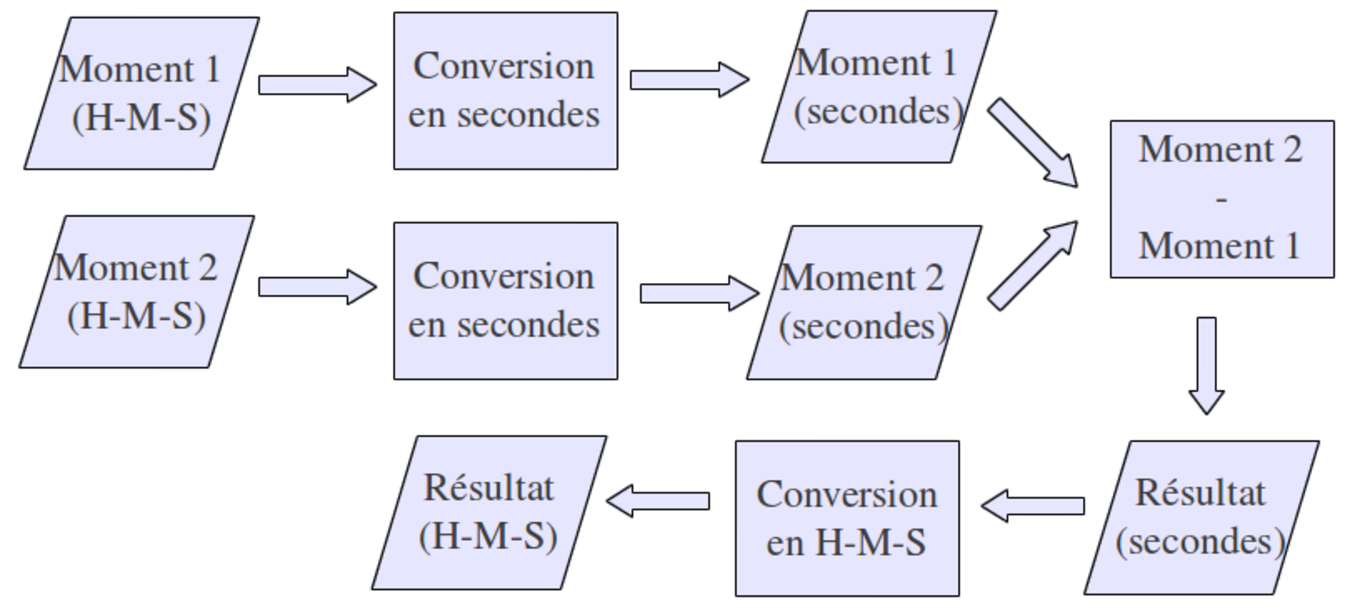
\includegraphics[width=0.8\textwidth]{image/module-conversion}
	\end{center}
\end{frame}

\subsubsection{Conversion en secondes}

\begin{frame}{Écart entre 2 moments}
	Une des sous-tâches est donc la conversion en secondes
	d'un moment exprimé en heures-minutes-secondes
	(h-m-s). 
	
	\bigskip
	
	Il nous faut adapter la solution trouvée pour
	l'exercice du chapitre sur les algorithmes séquentiels
	car il n'est pas question ici que les données soient
	lues ni que le résultat soit écrit~; 
	
	\bigskip
	
	l'interaction ne
	se fait pas avec l'utilisateur mais avec le module
	principal qui va l'utiliser.
\end{frame}

\begin{frame}{Écart entre 2 moments}
	La première question à se poser est donc celle des paramètres~:

	\bigskip
	
	\begin{itemize}
	\item 
		Quelles sont les données dont a besoin l'algorithme
		pour travailler ?
	\item 
		Quels résultats fournit-il ?
	\end{itemize}
\end{frame}

\begin{frame}{Écart entre 2 moments}
	Dans notre cas, la réponse est simple~:

	\bigskip
	
	\begin{itemize}
	\item {
		Les données sont le moment à convertir en secondes. 
		
		Ce moment est
		représenté par trois entiers~: les heures, les minutes et les secondes
		;}
	\item {
		Le résultat est le moment converti en secondes. 
		
		Il est représenté par un entier.}
	\end{itemize}
\end{frame}

\begin{frame}{Écart entre 2 moments}
	Lorsque le résultat est représenté par une seule donnée, on a le choix
	entre un paramètre en sortie~:

	\bigskip
	
	\cadre{
	\begin{pseudo}
		\LComment Affiche trois entiers~: des heures, des minutes et des secondes et sort le nombre de secondes correspondant.
		\ModuleSign{hmsVersSec}{h\In, m\In, s\In, secondes\Out~: entiers}{}
	\end{pseudo}
	}
	
	\bigskip
	
	ou une valeur de retour~:

	\bigskip
	
	\cadre{
	\begin{pseudo}
		\LComment Affiche trois entiers~: des heures, des minutes et des secondes et retourne le nombre de secondes correspondant.
		\ModuleSign{hmsVersSec}{h\In, m\In, s\In~: entiers}{entier}
	\end{pseudo}
	}
\end{frame}

\begin{frame}{Écart entre 2 moments}
		Dans de pareils cas, 
	on privilégie souvent la valeur de retour car cela
	facilite l'écriture lors de l'appel.

	\bigskip
	
	L'algorithme s'écrit alors~:

	\bigskip
	
	\cadre{
	\begin{pseudo}
	\LComment Affiche trois entiers~: des heures, des minutes et des secondes 
	\LComment et retourne le nombre de secondes correspondant.
		\Module{hmsVersSec}{h\In, m\In, s\In~: entiers}{entier}
			\Decl secondes~: entier \RComment {À déclarer puisque ce n'est pas un paramètre}
			\Let secondes \Gets  h * 3600 + m * 60 + s
			\Return secondes
		\EndModule
	\end{pseudo}
	}
\end{frame}

\begin{frame}{Écart entre 2 moments}
	ou de manière équivalente mais plus concise~:

	\bigskip
	
	\cadre{
	\begin{pseudo}
	\LComment Affiche trois entiers~: des heures, des minutes et des secondes 
	\LComment et retourne le nombre de secondes correspondant.
		\Module{hmsVersSec}{h\In, m\In, s\In~: entiers}{entier}
			\Return h * 3600 + m * 60 + s
		\EndModule
	\end{pseudo}
	}
\end{frame}

\subsubsection{Conversion en heures-minutes-secondes}

\begin{frame}{Conversion en heures-minutes-secondes}
	À la fin de notre algorithme, il nous faudra reconvertir un résultat
	exprimé en secondes sous la forme heures-minutes-secondes. 
	
	\bigskip
	
	À nouveau,
	on a déjà résolu ce problème dans le chapitre sur les algorithmes
	séquentiels. 
	
	\bigskip
	
	Mais il faut l'adapter à
	l'usage de paramètres.
\end{frame}

\begin{frame}{Conversion en heures-minutes-secondes}
	\begin{itemize}
	\item {
		Quelles sont les données ? 
		
		Une seule, le moment exprimé en secondes}
		
	\bigskip
	
	\item {
		Quels sont les résultats calculés par le module ? 
		
		Ce même moment exprimé
		en heures-minutes-secondes. 
		
		Trois entiers sont requis ce qui fait que
		le choix entre un paramètre en sortie et une valeur de retour ne se
		pose pas ici~; 
		
		impossible d'utiliser une valeur de
		retour (qui doit être unique)~; 
		
		on doit utiliser des paramètres en
		sortie.}
	\end{itemize}
\end{frame}

\begin{frame}{Conversion en heures-minutes-secondes}
	Ce qui donne~:

	\bigskip
	
	\cadre{
	\begin{pseudo}
		\LComment Affiche un nombre de secondes et sort les heures, les minutes et les secondes correspondant.
		\Module{secVersHMS}{secondes\In, s\Out, m\Out, s\Out~: entiers}{}
			\Let h \Gets secondes DIV 3600
			\Let m \Gets (secondes MOD 3600) DIV 60
			\Let s \Gets secondes MOD 60
		\EndModule
	\end{pseudo}
	}
\end{frame}

\subsubsection{Solution}

\begin{frame}{Solution}
	À présent, on a tout pour écrire la solution à notre problème

	\bigskip
	
	\cadre{
	\begin{pseudo}
		\LComment Lit deux moments (h-m-s) et affiche le moment de la différence entre les deux.
		\Module{différenceEntreHeures}{}{} \RComment Pas de paramètres !
			\Decl h1, m1, s1, h2, m2, s2~: entiers \RComment Les 2 moments à soustraire
			\Decl secondes1, secondes2~: entiers \RComment Ces 2 moments en secondes
			\Decl diffSecondes~: entier \RComment La différence en secondes
			\Decl diffH, diffM, diffS~: entiers \RComment La différence en H-M-S
			\Read h1, m1, s1, h2, m2, s2
			\Let secondes1 \Gets hmsVersSec( h1, m1, s1 )
			\Let secondes2 \Gets hmsVersSec( h2, m2, s2 )
			\Let diffSecondes \Gets secondes2 – secondes1
			\Stmt secVersHMS( diffSecondes, diffH, diffM, diffS )
			\Write diffH, diffM, diffS
		\EndModule
	\end{pseudo}
	}
\end{frame}

\begin{frame}{Solution}
	Dans la solution ci-dessus, 
	quelle est ou quelles sont la/les variable(s) locale(s) 
	dont on pourrait se passer moyennant une réécriture de
	l'algorithme ?
\end{frame}

\subsection{Blocs}

\begin{frame}{Blocs}
	\begin{itemize}
	\item
	Un bloc est l’écriture d’une portion de module
	à l’extérieur de celui-ci. C’est un simple
	{\textit{déplacement}}
	de lignes de codes vers un autre endroit du texte de
	l'algorithme.
	
	\bigskip
	
	\item
	La raison de découper un module en blocs
	peut être le souci de clarifier un algorithme en le découpant en étapes
	bien distinctes.
	
	\bigskip
	
	\item
	Les variables
	d’un bloc ne sont donc pas des variables locales du bloc dans lequel
	elles apparaissent, mais bien des variables locales du module auquel
	appartient ce bloc.
	\end{itemize}
\end{frame}

\begin{frame}{Blocs}
	\begin{itemize}
	\item
	L’appel de l’exécution des instructions se trouvant
	dans un bloc est similaire à celui d’un module avec paramètres, on
	écrit simplement le nom du bloc comme s’il s’agissait d’une
	instruction.
	\end{itemize}
\end{frame}

\begin{frame}{Blocs}
	Pour exemple, le module additionnerFractions (première version dans le
	chapitre 3) pourrait se découper ainsi~:

	\bigskip
	
	\cadre{
	\begin{pseudo}
	\LComment Lit les contenus de 2 fractions et affiche leur somme
		\Module{additionnerFractions}{}{}
			\Stmt déclaration
			\Stmt lectureDonnées
			\Stmt calculs
			\Stmt écritureRésultat
		\EndModule
	\end{pseudo}
	}
\end{frame}

\begin{frame}{Blocs}
	\cadre{
	\begin{pseudo}
	\Block{déclaration}
		\Decl num1, den1, num2, den2, numRes, denRes~: entiers
	\EndBlock
	\end{pseudo}
	}

	\bigskip
	
	\cadre{
	\begin{pseudo}
	\Block{lectureDonnées}
		\Read num1, den1, num2, den2
	\EndBlock
	\end{pseudo}
	}
\end{frame}

\begin{frame}{Blocs}
	\cadre{
	\begin{pseudo}
	\Block{calculs}
		\Let numRes \Gets num1 * den2 + num2 * den1
		\Let denRes \Gets den1 * den2
	\EndBlock
	\end{pseudo}
	}

	\bigskip
	
	\cadre{
	\begin{pseudo}
	\Block{écritureRésultat}
		\Write numRes, "/", denRes \RComment la fraction n'est pas simplifiée
	\EndBlock
	\end{pseudo}
	}
\end{frame}

\subsection{Qu'est-ce qu'un algorithme de qualité ?}

\begin{frame}{Algorithme de qualité}
	\begin{itemize}
	\item
	Nous voulons tous produire du code de qualité mais
	qu'est-ce que cette notion recouvre vraiment ?
	\item
	Qu'est-ce qui permet de juger de la qualité
	d'un code ? 
	\item
	De nombreux critères existent. 
	\end{itemize}
	
	\bigskip
	
	Citons ici,
	parmi les plus pertinents, ceux qui sont le plus liés à ce
	cours.
\end{frame}

\begin{frame}{Algorithme de qualité}
	\begin{itemize}
	\item
		La \textbf{validité}~: le code doit
	réaliser les tâches pour lesquelles 
	il a été écrit, même dans tous les
	cas particuliers imaginés.
	
	\bigskip
	
	\item 
		L'\textbf{extensibilité} (ou évolutivité)~:
	le code doit être écrit de telle sorte qu'un changement
	mineur dans le problème n'implique
	qu'un changement mineur dans le code.
	
	\bigskip
	
	\item
		La \textbf{réutilisabilité}~: c'est
	la capacité de réutiliser 
	un bout de code d’un projet dans un autre projet de 
	façon aisée et sûre.
	\end{itemize}
\end{frame}

\begin{frame}{Algorithme de qualité}
	\begin{itemize}
	\item
		La \textbf{lisibilité}~: 
		
	Au niveau global, on doit facilement comprendre la structure
	générale du code afin de pouvoir aisément comprendre où se trouve 
	la portion de	code qui nous intéresse. 
	
	Au niveau local, on doit pouvoir comprendre
	aisément chaque bout de code.
	
	\bigskip
	
	\item 
		L'\textbf{efficience}~: 
	ce critère s'intéresse à la bonne utilisation des
	ressources informatiques. Est-ce que le programme va tourner
	suffisamment vite, utiliser peu de mémoire ?
	\end{itemize}
\end{frame}

\section{Les variables structurées}
%\leconwithtoc

\subsection{Le type structuré}

\begin{frame}{types simple et structuré}
	\begin{itemize}
		\item
		Les variables de \code{types}
		dits «~\code{simples}~» ne peuvent
		contenir qu’une seule valeur à la fois  
		(entier, réel, booléen, caractère, chaine).
		
		\bigskip
	
		\item
		Cependant, certains types
		d’information consistent en un 
		regroupement de plusieurs données
		élémentaires.
		\begin{itemize}
			\item 
				une \textbf{date} est composée de trois éléments (le jour, le mois,
				l’année);
			\item {
				un \textbf{moment} de la journée est un triple d’entiers (heures,
				minutes, secondes)}
			\item {
				la localisation d’un \textbf{point} dans un plan nécessite 
				deux coordonnées cartésiennes (l’abscisse \textit{x} et
				l’ordonnée \textit{y}) ou polaires (le rayon \textit{r} et l’angle
				\textit{$\theta $})}
			\item {
				une \textbf{adresse }est composée de plusieurs données}
		\end{itemize}
		
	\end{itemize}
\end{frame}

\begin{frame}{type structuré}
	Pour stocker et manipuler de tels ensembles de données, nous utiliserons
	des \textbf{types structurés} ou \textbf{structures}.
	
	\bigskip
	
	\cadre{
	Une \code{structure} est donc un ensemble
	fini d’éléments pouvant être de types distincts. Chaque élément de cet
	ensemble, appelé \code{champ} de la structure, possède un nom unique.
	}
	
	\bigskip
	
	Noter qu’un champ d’une structure peut lui-même être une structure. 
	
	Par	exemple, une \textbf{carte d’identité} inclut parmi ses informations
	une \textbf{date} de naissance, l’\textbf{adresse} de son
	propriétaire (cachée dans la puce électronique!),\dots
\end{frame}

\subsection{Définition d'une structure}

\begin{frame}{Définition}
	La définition d’un type structuré adoptera le modèle suivant~:

	\bigskip
	
	\cadre{
	\begin{pseudo}
	\Struct{NomDeLaStructure}
		\Decl nomChamp1~: type1
		\Decl nomChamp2~: type2
		\Decl \dots
		\Decl nomChampN~: typeN
	\EndStruct
	\end{pseudo}
	}

	\bigskip
	
	\textit{nomChamp1}, \dots, \textit{nomChampN }
	sont les noms des différents champs de la structure, 
	et \textit{type1}, \dots, \textit{typeN} 
	les types de ces champs. 
	
	\bigskip
	
	Ces types sont 
	\begin{itemize}
	\item
	soit les types «~simples~» étudiés
	précédemment (entier, réel, booléen, caractère, chaine) 
	\item
	soit d’autres
	types structurés dont la structure aura été préalablement définie.
	\end{itemize}
\end{frame}

\begin{frame}{Exemple}
	Pour exemple, nous définissons ci-dessous trois
	types structurés que nous utiliserons souvent par la suite~:

	\bigskip
	
	\cadre{
	\begin{pseudo}
	\Struct{Date}
		\Decl jour~: entier
		\Decl mois~: entier
		\Decl année~: entier
	\EndStruct
	\end{pseudo}
	}
\end{frame}

\begin{frame}{Exemple}
	\cadre{
	\begin{pseudo}
	\Struct{Moment}
		\Decl heure~: entier
		\Decl minute~: entier
		\Decl seconde~: entier
	\EndStruct
	\end{pseudo}
	}

	\bigskip
	
	\cadre{
	\begin{pseudo}
	\Struct{Point}
		\Decl x~: réel
		\Decl y~: réel
	\EndStruct
	\end{pseudo}
	}

\end{frame}

\subsection{Déclaration d’une variable de type structuré}

\begin{frame}{Exemple}
	Une fois un type structuré défini, la
	déclaration de variables de ce type est identique à celle des variables
	simples. 
	
	\bigskip
	
	Par exemple~:

	\bigskip
	
	\cadre{
	\begin{pseudo}
	\Decl anniversaire, jourJ~: Date
	\Decl départ, arrivée, unMoment~: Moment
	\Decl a, b, centreGravité~: Point
	\end{pseudo}
	}
\end{frame}

\subsection{Utilisation des variables de type structuré}

\begin{frame}{Utilisation d'un champ}
	Pour accéder à l’un des champs d’une variable structurée, il faut mentionner
	le nom de ce champ ainsi que celui de la variable dont il fait partie.
	
	\bigskip
	
	Nous utiliserons la notation «~pointée~»~:
	
	\bigskip

	\cadre{
	\begin{pseudo}
	\Stmt nomVariable.nomChamp
	\end{pseudo}
	}
\end{frame}

\begin{frame}{Exemple}	
	\cadre{
	\begin{pseudo}
	\Let anniversaire.jour \Gets 15
	\Let anniversaire.mois \Gets 10
	\Let anniversaire.année \Gets 2014
	\Let arrivée.heure \Gets départ.heure + 2
	\Let centreGravité.x \Gets (a.x + b.x) / 2
	\end{pseudo}
	}
\end{frame}

\begin{frame}{Utilisation globale}
		On peut cependant, dans certains cas, utiliser
	une variable structurée de manière globale (c’est-à-dire d’une façon
	qui agit simultanément sur chacun de ses champs). 
	
	\bigskip
	
	Le cas le plus
	courant est l’affectation interne entre deux variables structurées de
	même type, par exemple~:

	\bigskip
	
	\cadre{
	\begin{pseudo}
	\Let arrivée \Gets départ
	\end{pseudo}
	}

	\bigskip
	
	qui résume les trois instructions suivantes~:

	\bigskip
	
	\cadre{
	\begin{pseudo}
	\Let arrivée.heure \Gets départ.heure
	\Let arrivée.minute \Gets départ.minute
	\Let arrivée.seconde \Gets départ.seconde
	\end{pseudo}
	}
\end{frame}

\begin{frame}{Paramètre d'un module}
	Une variable structurée peut aussi être le
	paramètre d’un module, et un module peut également renvoyer une
	«~valeur~» de type structuré. 
	
	\bigskip
	
	Par exemple, l’entête d’un module
	renvoyant le nombre de secondes écoulées entre une heure de départ et
	d’arrivée serait~:

	\bigskip
	
	\cadre{
	\begin{pseudo}
	\ModuleSign{nbSecondesEcoulées}{ départ\In, arrivée\In~: Moment}{entier}
	\end{pseudo}
	}
\end{frame}

\begin{frame}{Lire et afficher}
	On pourra aussi lire ou afficher une variable structurée.

	\bigskip
	
	\cadre{
	\begin{pseudo}
	\Read unMoment
	\Write unMoment
	\end{pseudo}
	}
\end{frame}

\begin{frame}{Comparaison}
	On ne peut pas utiliser les opérateurs de comparaison ({\textless}, {\textgreater}) pour
	comparer des variables structurées. 
	
	\bigskip
	
	En effet, s’il est naturel de vouloir comparer des dates ou des moments,
	comment définir une relation d’ordre avec les points du plan ou avec
	des cartes d’identités ?

	\bigskip
	
	Si le besoin de comparer des variables
	structurées se fait sentir, il faudra dans ce cas écrire des modules de
	comparaison adaptés aux structures utilisées.
\end{frame}

\begin{frame}{Assignation globale}
	Par facilité d'écriture, on peut assigner tous les champs en une 
	fois via des «~\{\}~». 
	
	\bigskip
	
	Exemple~:

	\bigskip
	
	\cadre{
	\begin{pseudo}
	\Let anniversaire \Gets \{1, 9, 1989\}
	\end{pseudo}
	}
\end{frame}

\subsection{Exemple d’algorithme}

\begin{frame}{Exemple}	
	Le module ci-dessous reçoit en paramètre deux dates ; 
	
	la valeur renvoyée est 
	\begin{itemize}
	\item
	–1 si la première date est antérieure à la deuxième, 
	\item
	0 si les deux	dates sont identiques 
	\item
	1 si la première date est postérieure à la
	deuxième.
	\end{itemize}
\end{frame}

\begin{frame}{Exemple}	
		\cadre{
	\begin{pseudo}
	\Module{comparerDates}{date1\In, date2\In~: Date}{entier}
		\Decl résultat~: entier
		\Let  résultat \Gets -1
		\RComment valeur choisie par défaut
		\If{date1.année ${\geq}$ date2.année}
			\If{date1.année $>$ date2.année}
				\Let  résultat \Gets 1
			\Else \RComment les années sont identiques
				\If{date1.mois ${\geq}$ date2.mois}
					\If{date1.mois $>$ date2.mois}
						\Let  résultat \Gets 1
					\Else \RComment les années et les mois sont identiques
						\If{date1.jour ${\geq}$ date2.jour}
							\If{date1.jour $>$ date2.jour}
								\Let  résultat \Gets 1
							\Else \RComment les années, les mois et les jours sont identiques
								\Let  résultat \Gets 0
							\EndIf
						\EndIf
					\EndIf
				\EndIf
			\EndIf
		\EndIf
		\Return résultat
	\EndModule
	\end{pseudo}
	}
\end{frame}

\section{Les boucles}
%\leconwithtoc

\subsection{La notion de travail répétitif}

\begin{frame}{La notion de travail répétitif}
	\begin{itemize}
		\item
		Les ordinateurs révèlent tout leur potentiel dans leur capacité à
		répéter inlassablement les mêmes tâches. 
	\item
		Si on veut faire effectuer un travail répétitif, 
		il faut indiquer deux choses~:
		
		\begin{enumerate}
			\item Le travail à répéter
			\item La manière de continuer la répétition 
				ou de l'arrêter.
		\end{enumerate}

	\end{itemize}
\end{frame}

\begin{frame}{Exemple 1}
	Pour traiter des dossiers, on dira quelque chose
	comme «~tant qu'il reste un dossier à traiter, le
	traiter~» ou encore «~traiter un dossier puis passer au suivant
	jusqu'à ce qu'il n'en reste plus à traiter~».

	\begin{itemize}
	\item la tâche à répéter est : «~traiter un dossier~»
	\item on indique qu'on doit continuer s'il
		reste encore un dossier à traiter
	\end{itemize}
	
	\bigskip

	\textbf{Remarque :} On aurait aussi pu le formuler ainsi : «~traiter un
	dossier et passer au suivant jusqu'à ce
	qu'il n'en reste plus~»
\end{frame}

\begin{frame}{Exemple 2}
	Pour calculer la cote finale de tous les étudiants,
	on aura quelque chose du genre «~Pour tout étudiant, calculer sa
	cote~»

	\begin{itemize}
	\item 
		La tâche à répéter est : «~calculer la cote d'un
		étudiant~»
	\item 
		On indique qu'on doit le faire pour tous les étudiants.
		On doit donc commencer par le premier, passer à chaque fois au suivant
		et s'arrêter quand on a fini le dernier.
	\end{itemize}
\end{frame}

\begin{frame}{Exemple 3}
	Pour afficher tous les nombres de 1 à 100, on aura
	«~Pour tous les nombres de 1 à 100, afficher ce nombre~»

	\begin{itemize}
	\item
		La tâche à répéter est : «~afficher un nombre~»
	\item 
		On indique qu'on doit le faire pour tous les nombres de
		1 à 100. On doit donc commencer avec 1, passer à chaque fois au nombre
		suivant et s'arrêter après avoir affiché le nombre
		100.
	\end{itemize}
\end{frame}

\begin{frame}{Attention}
	\textbf{Attention} ! Comprenez bien que c'est toujours
	la même tâche qui est exécutée mais pas avec le même effet à chaque
	fois. Ainsi, on traite un dossier mais à chaque fois un différent; on
	affiche un nombre mais à chaque fois un différent. 
	
	Voyons comment	y arriver en logique.
\end{frame}

\subsection{Structures itératives}

\subsubsection{«~tant que~»}

\begin{frame}{Tant que}
	Le «~tant que~» est une structure qui demande à
	l'exécutant de répéter une tâche (une ou plusieurs
	instructions) tant qu'une condition donnée est vraie.

	\bigskip

	\cadre{
		\begin{pseudo}
		\While{condition}
			\Stmt séquence d’instructions à exécuter
		\EndWhile
		\end{pseudo}
	}

\end{frame}

\begin{frame}{Tant que}
	\begin{itemize}
		\item
			Comme pour la structure \code{si}, la \code{condition} est
			une expression à valeur booléenne.
		\item
			Dans ce type de structure, il faut
			qu’il y ait dans la séquence d’instructions comprise entre
			\code{tant que} et \code{fin tant que} au moins une
			instruction qui modifie une des composantes de la condition de telle
			manière qu’elle puisse devenir \textbf{fausse} à un moment donné.
		\item 
			Dans le cas contraire, la condition reste indéfiniment vraie et la boucle va
			tourner sans fin, c'est ce qu'on appelle une \textbf{boucle infinie}.
		\item
			Si la condition est fausse dès le début, 
			la tâche n'est jamais exécutée.
	\end{itemize}
\end{frame}

\begin{frame}{Tant que}
	\begin{figure}[h]
		\centering
		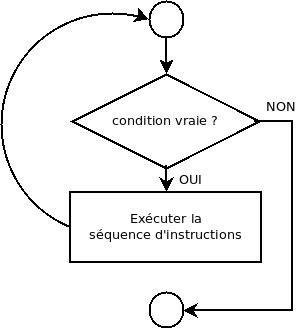
\includegraphics[width=0.5\textwidth]{image/boucle-tq}
		\caption{Ordinogramme de la boucle "tant-que"}
		\label{fig:boucle-tq}
	\end{figure}
\end{frame}

\subsubsection{«~faire – jusqu'à ce que~»}

\begin{frame}{«~faire – jusqu'à ce que~»}
	Cette structure est très proche du «~tant que~» 
	à deux différences près :
	
	\begin{enumerate}
		\item {
			Le test est fait à la fin et pas au début. La tâche est donc toujours
			exécutée au moins une fois. }
		\item {
			On donne la condition pour arrêter et pas pour continuer; il
			s'agit d'une différence mineure.}
	\end{enumerate}

	\bigskip
	
	\cadre{
		\begin{pseudo}
		\Repeat
			\Stmt séquence d’instructions à exécuter
		\Until{condition}
		\end{pseudo}
	}
\end{frame}

\begin{frame}{«~faire – jusqu'à ce que~»}
	\begin{itemize}
		\item 
			la séquence d’instructions comprise entre
			\code{faire} et \code{jusqu'a ce que} 
			contienne au moins une instruction qui modifie la condition de
			telle manière qu’elle puisse devenir \textbf{vraie} à un moment donné
			pour arrêter l'itération. 
	\end{itemize}
\end{frame}

\begin{frame}{«~faire – jusqu'à ce que~»}
	\begin{figure}[h]
	\centering
	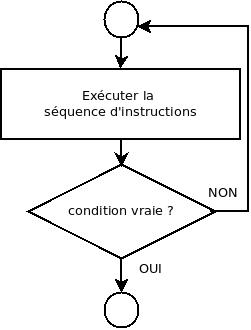
\includegraphics[width=0.4\textwidth]{image/boucle-faire}
	\caption{Ordinogramme de la boucle "faire – jusqu'à ce que"}
	\label{fig:boucle-faire}
	\end{figure}
\end{frame}

\subsubsection{«~pour~»}

\begin{frame}{«~pour~»}
	\begin{itemize}
		\item
		Ici, on va plutôt indiquer \textbf{combien de fois} la tâche doit être
		répétée. 
		\item
		Cela se fait au travers d'une
		\textbf{variable de contrôle} dont la valeur va évoluer à partir
		d'une valeur de départ jusqu'à une
		valeur finale.
	\end{itemize}
\end{frame}

\begin{frame}{«~pour~»}
	\cadre{
		\begin{pseudo}
		\For{variable \K{de} début \K{à} fin [\K{par} pas]}
			\Stmt séquence d’instructions à exécuter
		\EndFor
		\end{pseudo}
	}

	\begin{itemize}
		\item
		Dans ce type de structure, \code{debut}, \code{fin} et \code{pas}
		peuvent être des constantes, des variables ou des expressions (le plus
		souvent à valeurs entières mais on admettra parfois des réels). 
		\item
		Le \code{pas} est facultatif, et généralement omis (dans ce cas, sa valeur 
		par défaut est 1). 
		\item
		Ce pas est parfois négatif, dans le cas
		d'un compte à rebours, par exemple
		\code{pour n de 10 a 1 par -1}.
	\end{itemize}
\end{frame}

\begin{frame}{«~pour~»}
	\begin{itemize}
		\item
		Quand le \code{pas} est positif, la boucle s'arrête
		lorsque la variable dépasse la valeur de \code{fin}.
		\item
		Par contre, avec
		un \code{pas} négatif, la boucle s'arrête lorsque la
		variable prend une valeur plus petite que la valeur de \code{fin}
	\end{itemize}
\end{frame}

\begin{frame}{«~pour~»}
	\begin{figure}[h]
		\centering
		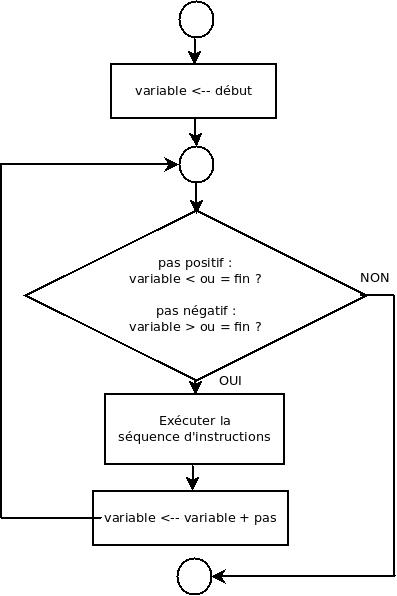
\includegraphics[width=0.4\textwidth]{image/boucle-pour}
		\caption{Ordinogramme de la boucle "pour"}
		\label{fig:boucle-pour}
		\end{figure}
\end{frame}

\begin{frame}{Attention}
	\begin{itemize}
		\item
		On considérera
		qu’au cas (à éviter) où \code{debut} est strictement supérieur à
		\code{fin} et le \code{pas} est positif, la séquence d’instructions
		n’est jamais exécutée (mais ce n’est pas le cas dans tous les langages
		de programmation !). 
		\item
		Idem si \code{debut} est strictement inférieur à
		\code{fin} mais avec un \code{pas} négatif.
		\item
		Attention de ne pas modifier dans la séquence d’instructions une des
		variables de contrôle \code{debut}, \code{fin} ou \code{pas} !
	\end{itemize}
\end{frame}

\begin{frame}{Attention}
	\begin{itemize}
		\item
		Il est aussi fortement déconseillé de modifier «~manuellement~» la
		\code{variable} de contrôle au sein de la boucle
		\code{pour}. Il ne faut pas l’initialiser en début de boucle,
		et ne pas s’occuper de sa modification, l’instruction 
		\code{variable} $\leftarrow$ \code{variable} + \code{pas} 
		étant automatique et implicite à chaque étape de la
		boucle.
		\item
		Il est aussi déconseillé d’utiliser \code{variable} à la
		sortie de la structure \code{pour} sans lui affecter une
		nouvelle valeur (son contenu pouvant varier selon le langage de
		programmation).
	\end{itemize}
\end{frame}


\begin{frame}{Exemples~}
	\cadre{
	\begin{pseudo}
	\Stmt \K{pour} i \K{de} 0 \K{à} 2 \K{faire} \RComment La boucle est exécutée 3 fois.
	\Stmt \K{pour} i \K{de} 2 \K{à} 0 \K{faire} \RComment La boucle n'est pas exécutée.
	\Stmt \K{pour} i \K{de} 1 \K{à} 10 \K{par} -1 \K{faire} \RComment La boucle n'est pas exécutée.
	\Stmt \K{pour} i \K{de} 1 \K{à} 1 \K{par} 5 \K{faire} \RComment La boucle est exécutée 1 fois.
	\end{pseudo}
	}
\end{frame}	

\subsection{Quel type de boucle choisir ?}

\begin{frame}{Quelle boucle choisir ?}
	\begin{itemize}
		\item
		En pratique, il est possible d’utiliser systématiquement la boucle 
		\code{tant que} qui peut s’adapter à toutes les situations. 
		\item
		Cependant, il est plus clair d’utiliser la boucle \code{pour} 
		dans les cas où le nombre d’itérations est fixé et connu à l’avance 
		\item
		La boucle \code{faire} convient quant à elle
		dans les cas où le contenu de la boucle doit être parcouru au moins une
		fois, 
		
		alors que dans \code{tant que}, 
		le nombre de parcours peut être nul si la condition initiale est fausse. 
	\end{itemize}
\end{frame}

\begin{frame}{Quelle boucle choisir ?}
	\begin{figure}[h]
	\centering
	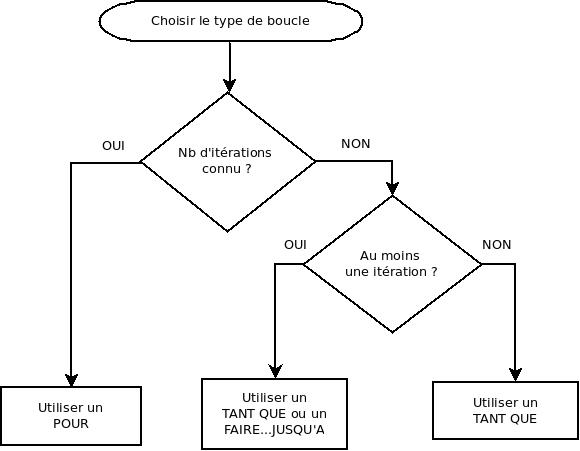
\includegraphics[width=0.7\textwidth]{image/boucle-choixtype}
	\caption{Quel type de boucle choisir ?}
	\label{fig:boucle-choix}
	\end{figure}
\end{frame}
	
\subsection{Exemples}

\subsubsection{Exemple 1 -- Compter de 1 à 10}

\begin{frame}{Compter de 1 à 10}
	Imaginons qu'on veuille afficher tous les nombres de 1 à 10. 
	
	On va évidemment \textbf{rejeter} cette première solution :

	\cadre{
	\begin{pseudo}
	\LComment Affiche les nombres de 1 à 10.
	\Module{compterJusque10}{}{} \RComment une mauvaise solution !
	\Write 1
	\Write 2
	\Write 3
	\Write 4
	\Write 5
	\Write 6
	\Write 7
	\Write 8
	\Write 9
	\Write 10
	\EndModule
	\end{pseudo}
	}
\end{frame}

\begin{frame}{Compter de 1 à 10}
	\begin{itemize}
	\item
	Non seulement c'est long à écrire 
	(imaginer l'algorithme pour afficher les nombres de 1 à 10000 !) 
	mais c'est très peu souple.
	\item
	Cela ne fonctionne que pour 10 : il faut modifier l'algorithme pour
	un autre comptage.
	\item
	La boucle va nous permettre
	d'obtenir un algorithme qui s'adapte
	à la limite du décompte.
	\end{itemize}
\end{frame}
	
\begin{frame}{Compter de 1 à 10}
	Posons-nous les bonnes questions pour déterminer la boucle :

	\begin{itemize}
	\item 
		Quelle est la tâche à répéter ? Afficher un nombre.
	\item 
		Comment savoir si on continue ? On arrête quand «~10~» est affiché.
	\item 
		Comment afficher à chaque fois un nombre différent ? 
		Au travers d'une variable qui prendra toutes les valeurs de 1 à 10. 
		Il faut donc ajouter dans le corps de la
		boucle une incrémentation de la variable
	\end{itemize}
\end{frame}

\begin{frame}{Compter de 1 à 10}
	Ce qui donne :

	\cadre{
	\begin{pseudo}
	\LComment A les nombres de 1 à 10.
	\Module{compterJusque10}{}{} \RComment version avec tant que
		\Decl nb : entier
		\Let nb \Gets 1 \RComment c'est le premier nombre à afficher
		\While{nb $\leq$ 10} \RComment tant que le nb à afficher est toujours bon
			\Write nb \RComment on affiche la valeur de la variable nb
			\Let nb \Gets nb + 1 \RComment on passe au nombre suivant
		\EndWhile
	\EndModule
	\end{pseudo}
	}
\end{frame}

\begin{frame}{Compter de 1 à 10}
	Mais ici, on pourrait aussi l'écrire avec un «~pour~» vu qu'on
	connait exactement le nombre d'exécutions de la boucle (10). 
	
	\medskip
	
	La variable de contrôle va évoluer de 1 à 10 ce qui tombe bien car
	c'est justement le nombre à afficher à chaque fois.
	
	\medskip

	\cadre{
	\begin{pseudo}
	\LComment Affiche les nombres de 1 à 10.
	\Module{compterJusque10}{}{} \RComment version avec pour
		\Decl nb : entier
		\For{nb \K{de} 1 \K{à} 10} \RComment par défaut le pas est de 1
			\Write nb 
		\EndFor
	\EndModule
	\end{pseudo}
	}
\end{frame}

\subsubsection{Exemple 2 -- Compter de 1 à beaucoup}

\begin{frame}{Compter de 1 à beaucoup}
	Dans l'exercice précédent, on a
	affirmé que la boucle pouvait s'adapter à la limite du
	décompte. Montrons-le ! 
	
	\bigskip
	
	Supposons qu'on veuille
	afficher les nombres de 1 à $n$ où $n$ est une valeur 
	donnée par l'utilisateur.

	\bigskip

	Rien de plus simple, il suffit de lire cette
	valeur au début et de l'utiliser comme limite de boucle
\end{frame}

\begin{frame}{Compter de 1 à beaucoup}
	\cadre{
	\begin{pseudo}
	\LComment Lit un nombre et affiche les nombres de 1 à ce nombre.
	\Module{afficherN}{}{} 
		\Decl nb, n : entier
		\Read n
		\For{nb \K{de} 1 \K{à} n} 
			\Write nb 
		\EndFor
	\EndModule
	\end{pseudo}
	}
\end{frame}

\begin{frame}{Compter de 1 à beaucoup}
	Que se passe-t-il si l'utilisateur entre une valeur négative ?
	
	\bigskip
	
	Comment améliorer le code pour que le programme
	le signale à l'utilisateur ?
\end{frame}

\subsubsection{Exemple 3 -- Afficher les nombres pairs}

\begin{frame}{Afficher les nombres pairs}
	Cette fois-ci on affiche uniquement les nombres 
	\textbf{pairs} jusqu'à la limite $n$.
	
	\bigskip
	
	\textbf{Exemple} : 
	les nombres pairs de $1$ à $10$ sont : $2$, $4$, $6$, $8$, $10$.
	
	\bigskip
	
	Notez que $n$ peut être impair. Si $n$ vaut $11$, 
	l'affichage est le même que pour $10$.

	\bigskip

	Est-ce qu'on peut utiliser un «~pour~» ? 
\end{frame}

\begin{frame}{Afficher les nombres pairs}
	Est-ce qu'on peut utiliser un «~pour~» ? 

	\bigskip
	
	Oui. De 1 à $n$, il y a exactement «~$n$ DIV $2$~» nombres à afficher. 
	
	\bigskip
	
	La difficulté vient du lien à faire entre la variable de
	contrôle et le nombre à afficher.
\end{frame}

\begin{frame}{Afficher les nombres pairs}

	\textbf{Solution 1} : 
	on garde le lien entre la variable de contrôle 
	et le nombre à afficher. 
	Dans ce cas, on commence à $2$ et le pas doit être de $2$.

	\bigskip
	
	\cadre{
	\begin{pseudo}
	\LComment Lit un nombre et affiche les nombres pairs jusqu'à ce nombre.
	\Module{afficherPair}{}{} 
		\Decl nb, n : entier
		\Read n
		\RComment limite des nombres à afficher
		\For{nb \K{de} 2 \K{à} n \K{par} 2} 
			\Write nb 
		\EndFor
	\EndModule
	\end{pseudo}
	}
\end{frame}

\begin{frame}{Afficher les nombres pairs}
	\textbf{Solution 2} : 
	la variable de contrôle compte simplement le nombre d'itérations.
	
	Alors il faut calculer le nombre à afficher en fonction de la variable
	de contrôle (ici le double de celle-ci convient)

	\bigskip
	
	\cadre{
	\begin{pseudo}
	\LComment Lit un nombre et affiche les nombres pairs jusqu'à ce nombre.
	\Module{afficherPair}{}{} 
		\Decl i, n : entier
		\Read n
		\RComment limite des nombres à afficher
		\For{i \K{de} 1 \K{à} n DIV 2} 
			\Write 2 * i 
		\EndFor
	\EndModule
	\end{pseudo}
	}
\end{frame}

\subsection{Exemple 4 -- Afficher les premiers nombres pairs}

\begin{frame}{Afficher les premiers nombres pairs}
	Voici un problème proche du précédent : 
	on affiche cette fois les $n$ premiers nombres pairs.
	
	\bigskip
	
	\textbf{Exemple} : 
	les $10$ premiers nombres pairs sont : $2$, $4$, $6$, $8$, $10$, $12$, $14$, $16$, $18$, $20$.
	
	\bigskip
	
	Il est plus simple de partir de la solution 2 de l'exemple précédent
	en changeant simplement la valeur finale de la boucle.
\end{frame}

\begin{frame}{Afficher les premiers nombres pairs}

		\cadre{
		\begin{pseudo}
		\LComment Lit un nombre et affiche ce nombre de nombres pairs.
		\Module{afficherPair}{}{} 
			\Decl i, n : entier
			\Read n
			\RComment le nombre de nombres à afficher
			\For{i \K{de} 1 \K{à} n} 
				\Write 2 * i 
			\EndFor
		\EndModule
		\end{pseudo}
		}
\end{frame}

\subsubsection{Exemple 5 -- Somme de nombres}

\begin{frame}{Somme de nombres}
	On veut pouvoir calculer (et retourner)
	la somme d'une série de nombres donnés par
	l'utilisateur. 
	
	\bigskip
	
	Il faut d'abord se
	demander comment l'utilisateur va pouvoir indiquer
	combien de nombres il faut additionner ou quand est-ce que le dernier
	nombre à additionner a été entré. 
	
	\bigskip
	
	Voyons quelques possibilités.
\end{frame}

\begin{frame}{Somme de nombres}
	\textbf{Variante 1}~: 
	
	L'utilisateur indique le nombre de termes au départ.
	
	\cadre{
	\begin{pseudo}
	\LComment Lit des valeurs entières et retourne la somme des valeurs lues.
	\Module{sommeNombres}{}{entier} \RComment Variante 1
		\Decl nbValeurs : entier \RComment nb de valeurs à additionner
		\Decl valeur : entier \RComment un des termes de l'addition
		\Decl somme : entier \RComment la somme
		\Decl i : entier \RComment itérateur
		\Let somme \Gets 0 \RComment la somme se construit petit à petit. 0 au départ
		\Read nbValeurs
		\For{i \K{de} 1 \K{à} nbValeurs} 
			\Read valeur
			\Let somme \Gets somme + valeur 
		\EndFor
		\Return somme
	\EndModule
	\end{pseudo}
	}
\end{frame}

\begin{frame}{Somme de nombres}
	\textbf{Variante 2}~: 
		
	Après chaque nombre, 
	on demande à l'utilisateur s'il y a encore un nombre à additionner.

	\bigskip
	
	Ici, il faut chercher une solution différente
	car on ne connait pas au départ le nombre de valeurs à additionner et
	donc le nombre d'exécution de la boucle. 
	
	\bigskip
	
	On va devoir passer à un
	«~tant que~» ou un «faire - jusqu'à ce que». 
	
	\bigskip
	
	On peut
	envisager de demander en fin de boucle si il reste
	encore un nombre à additionner. 
\end{frame}

\begin{frame}{Somme de nombres}
	\cadre{
	\begin{pseudo}
	\LComment Lit des valeurs entières et retourne la somme des valeurs lues.
	\Module{sommeNombres}{}{entier} \RComment Variante 2a
		\Decl encore : booléen \RComment est-ce qu'il reste encore une valeur à additionner ?
		\Decl valeur : entier \RComment un des termes de l'addition
		\Decl somme : entier \RComment la somme
		\Let somme \Gets 0
		\Repeat 
			\Read valeur
			\Let somme \Gets somme + valeur 
			\Read encore
		\Until{NON encore}
		\Return somme
	\EndModule
	\end{pseudo}
	}
\end{frame}

\begin{frame}{Somme de nombres}
	Avec cette solution, on additionne au moins une valeur. 
	
	\bigskip
	
	Si on veut pouvoir tenir compte du
	cas très particulier où l'utilisateur ne veut
	additionner aucune valeur, il faut utiliser un «~tant que~» et donc
	poser la question avant d'entrer dans la boucle.
\end{frame}

\begin{frame}{Somme de nombres}
	\cadre{
	\begin{pseudo}
	\LComment Lit des valeurs entières et retourne la somme des valeurs lues.
	\Module{sommeNombres}{}{entier} \RComment Variante 2b
		\Decl encore : booléen \RComment est-ce qu'il reste encore une valeur à additionner ?
		\Decl valeur : entier \RComment un des termes de l'addition
		\Decl somme : entier \RComment la somme
		\Let somme \Gets 0
		\Read encore
		\While{encore} 
			\Read valeur
			\Let somme \Gets somme + valeur 
			\Read encore
		\EndWhile
		\Return somme
	\EndModule
	\end{pseudo}
	}
\end{frame}

\begin{frame}{Somme de nombres}
	\textbf{Variante 3}~:
	
	L'utilisateur entre une valeur spéciale pour indiquer la fin. 
	On parle de valeur \textbf{sentinelle}. 
	
	\bigskip
	
	Ceci n'est possible que si cette valeur \textbf{sentinelle} ne peut pas être
	un terme valide de l'addition. 
	
	\bigskip
	
	Par exemple, si on veut
	additionner des nombres positifs uniquement, la valeur -1 peut servir
	de valeur sentinelle. 
	
	\bigskip
	
	Mais sans limite sur les nombres à additionner
	(positifs, négatifs ou nuls) il n'est pas possible de
	choisir une sentinelle.
\end{frame}

\begin{frame}{Somme de nombres}
	Ici, on se base sur la valeur entrée pour décider si on continue ou pas. 
	
	\bigskip
	
	Il faut donc \textbf{toujours} effectuer un test
	après une lecture de valeur. 
	
	\bigskip
	
	C'est pour cela
	qu'il faut effectuer une lecture avant et une autre à
	la fin de la boucle.

\end{frame}

\begin{frame}{Somme de nombres}
	\cadre{
	\begin{pseudo}
	\LComment Lit des valeurs entières et retourne la somme des valeurs lues.
	\Module{sommeNombres}{}{entier} \RComment Variante 3
		\Decl valeur : entier \RComment un des termes de l'addition
		\Decl somme : entier \RComment la somme
		\Let somme \Gets 0
		\Read valeur
		\While{valeur ${\geq}$ 0} 
			\Let somme \Gets somme + valeur 
			\Read valeur \RComment remarquer l'endroit où on lit une valeur.
		\EndWhile
		\Return somme
	\EndModule
	\end{pseudo}
	}
\end{frame}

\begin{frame}{Somme de nombres}
	\textbf{Réflexions}~: 
	\begin{itemize}
	\item
		Quelle valeur sentinelle prendrait-on 
		pour additionner une série de cotes d'interrogations ? 
		Une série de températures ?
	\item
		Dans les solutions 2 et 3 on lit une variable booléenne. 
		Comment un programmeur pourrait-il réaliser 
		cette instruction de façon pratique ?		
	\end{itemize}
\end{frame}

\subsubsection{Exemple 6~: Suite des nombres pairs}

\begin{frame}{Suite des nombres pairs}
	Écrire l'algorithme qui affiche les $n$ premiers termes
	de la suite: $2$, $4$, $6$\dots
	
	\bigskip
	
	Puisqu'on doit écrire plusieurs nombres et qu'on sait exactement combien,
	on se tournera tout naturellement vers une boucle \K{pour}.

	\bigskip
	
	Le cas le plus simple est lorsque le nombre à afficher à l'étape $i$
	peut être calculé en fonction de $i$ seulement.
	
\end{frame}

\begin{frame}{Suite des nombres pairs}
	\cadre{
	\begin{pseudo}
	\For{i de 1 à n}
		\Write $f(i)$
	\EndFor
	\end{pseudo}
	}
\end{frame}

\begin{frame}{Suite des nombres pairs}

	Dans ce cas, la fonction est $f(i)=2*i$
	(Si vous n'êtes pas convaincu, vérifiez qu'à l'étape $1$ on affiche $2$,
	à l'étape $2$ on affiche $4$ \dots)
	
	\bigskip

	\cadre{
	\begin{pseudo}
	\Module{nombrePair}{n\In: entier}{}
		\Decl i : entier
		\For{i de 1 à n}
			\Write 2 * i
		\EndFor
	\EndModule
	\end{pseudo}
	}
\end{frame}

\begin{frame}{Suite des nombres pairs}
	Parfois, il est difficile (voire impossible) de trouver $f(i)$.
	
	\bigskip
	
	On suivra alors une autre approche qui revient à calculer un nombre
	à afficher à partir du nombre précédemment affiché
	(ou, plus exactement, de calculer le suivant à partir du nombre
	qu'on vient d'afficher).
	La structure générale est alors

	\bigskip
	
	\cadre{
	\begin{pseudo}
	\Let nb \Gets \textit{\{1\up{ère} valeur à afficher\}}
	\For{i de 1 à n}
		\Write nb
		\Let nb \Gets \textit{\{calculer ici le nb suivant\}}
	\EndFor
	\end{pseudo}
	}
\end{frame}

\begin{frame}{Suite des nombres pairs}
	Dans l'exemple de la suite paire, le 1\up{er} nombre à afficher est $2$
	et le nombre suivant se calcule en ajoutant $2$ au nombre courant.

	\bigskip
	
	\cadre{
	\begin{pseudo}
	\Module{suite1}{n\In: entier}{}
		\Decl nb, i : entiers
		\Let nb \Gets 2
		\For{i de 1 à n}
			\Write nb
			\Let nb \Gets nb + 2
		\EndFor
	\EndModule
	\end{pseudo}
	}
\end{frame}

\begin{frame}{Suite des nombres pairs}
	On remarque que, lors du dernier passage dans la boucle,
	on calcule une valeur qui ne sera pas affichée.
	Cette petite perte de temps est dommage mais négligeable
	et permet de garder une structure claire et générale à la solution.

	\bigskip
	
	Dans certains cas,
	il n'est pas possible de déduire directement le nombre suivant
	en connaissant juste le nombre précédent.
	Prenons un exemple pour l'illustrer.
\end{frame}

\subsection{Exemple 7~: 3 pas en avant, 2 pas en arrière} 

\begin{frame}{3 pas en avant, 2 pas en arrière} 
	Écrire l'algorithme qui affiche les $n$ premiers termes
	de la suite: $1$, $2$, $3$, $4$, $3$, $2$, $3$, $4$, $5$, $4$, $3$\dots

	\bigskip
	
	Si on vient d'écrire, disons un $3$,
	impossible sans information supplémentaire,
	de connaitre le nombre suivant.
	
	\bigskip
	
	Il faudrait savoir si on est en phase d'avancement ou de recul
	et combien de pas il reste à faire dans cette direction.

	\bigskip
	
	Ajoutons des variables pour retenir l'\textbf{état} où on est.
\end{frame}

\begin{frame}{3 pas en avant, 2 pas en arrière} 
	\cadre{
	\begin{pseudo}
	\Module{suite3Avant2Arrière}{n\In: entier}{} 
		\Decl nb, nbPasRestants, direction, i : entiers
		\Let nb \Gets 1
		\Let nbPasRestants \Gets 3 \RComment 3 pas
		\Let direction \Gets 1 \RComment en avant
		\For{i de 1 à n}
			\Write nb
			\Let nb \Gets nb + direction \RComment faire un pas dans la bonne direction
			\Let nbPasRestants \Gets nbPasRestants - 1
			\If{nbPasRestants $=$ 0} \RComment il est temps de changer de direction
				\Let direction \Gets -direction
				\If{direction $=$ 1}
					\Let nbPasRestants \Gets 3 
				\Else 
					\Let nbPasRestants \Gets 2
				\EndIf
			\EndIf
		\EndFor
	\EndModule
	\end{pseudo}
	}
\end{frame}

\begin{frame}{3 pas en avant, 2 pas en arrière} 
	On obtient un algorithme plus long 
	mais qui respecte toujours le schéma vu.

	\bigskip
	
	\textbf{Un conseil}~: essayez de respecter ce schéma 
	et vous obtiendrez plus facilement un algorithme
	correct et lisible, également dans les cas particuliers.
\end{frame}


% ====== Second quadrimestre


\section*{Annexe}
\begin{frame}{Crédits}
Ce document a été produit avec les outils suivants
\begin{itemize}
\item {\small Les distributions \sigle{\emph{Ubuntu}} et/ou \sigle{\emph{debian}} 
du système d'exploitation \sigle{\emph{Linux}}}
\item {\small \sigle{\emph{LaTeX}}/\sigle{\emph{Beamer}} comme système d'édition}
\item {\small \sigle{\emph{Git}} et \sigle{\emph{GitHub}} pour la gestion des versions et le suivi des corrections}
\item {\small Les outils \sigle{\emph{make}}, \sigle{\emph{rubber}}, \sigle{\emph{pdfnup}}, \dots}
\end{itemize}
\medskip
Il est proposé sous licence 
\begin{footnotesize}
\begin{center}
\textit{Creative Commons Paternité - Partage à l'Identique 2.0 Belgique}
\\\code|http://creativecommons.org/licenses/by-sa/2.0/be/|
\end{center}
\end{footnotesize}
\end{frame}

\end{document} 
 
